\documentclass[a4paper,12pt]{article}

\usepackage[utf8]{inputenc}
\usepackage[top=3cm, bottom=3cm, left=3cm, right=3cm]{geometry}
\usepackage{amsmath} % For bmatrix and others
\usepackage{enumitem}
\usepackage{tikz}
\usetikzlibrary{quantikz}
\usepackage{hyperref}

\newcommand{\exercise}[1]{\paragraph{Exercise #1}}
\newcommand{\la}{\langle}
\newcommand{\ra}{\rangle}

\begin{document}

    \begin{titlepage}
        \begin{center}
            \large Exercise solutions for\\ Quantum Computation and Quantum Information\\
            by Michael A. Nielsen \& Isaac L. Chuang\\[1.5cm]
            D. G. O.
        \end{center}
    \end{titlepage}

    \newpage

    \section*{Preface}

    The solutions are original, except where there is a citation. The quantum circuits were made using Quantikz\cite{kay2018tutorial}. The solutions here might be incorrect, use it at your own risk. If you find any error, please contact me.

    \newpage

    \section{Introduction and overview}

    \setcounter{subsection}{3}
    \subsection{Quantum algorithms}

    \setcounter{subsubsection}{3}
    \subsubsection{The Deutsch -- Jozsa algorithm}

    \exercise{1.1}

    Let $n$ be the number of bits, $m$ the number of samples Alice asks from Bob. Let $p$ be the probability, that Bob will create a constant function. After $m$ samples, Alice will determine, that the function is constant with probability $q$, that the function is constant, and she will determine, that the function is balanced with probability $(1 - q)$ if all reply bits are the same. If she sees the reply bits are not the same, she will determine that the function is balanced.

    In this case, the probability, that Alice will get the correct answer is
    \begin{equation}
      1 - \epsilon = p P_{\textrm{c}} + (1 - p) P_{\textrm{b}}\ \textrm{,}
    \end{equation}

    \noindent
    where $P_{\textrm{c}}$ is the probability, that Alice gets the right answer if the function is constant, and $P_{\textrm{b}}$ is the probability, that Alice gets the right answer if the function is balanced.

    If the function is constant, Alice will always gets the same bits, and so she will say the function is constant with $q$ probability: $P_{\textrm{c}} = q$.

    If the function is balanced, the probability that the reply bits will be all zeroes or all ones for $m$ randomly choosen function arguments from any random balanced function is
    \begin{equation}
      r = \frac{2\ {{n - m}\choose{n / 2}}}{{{n}\choose{n / 2}}}\ \textrm{,}
    \end{equation}

    \noindent
    because there ${{n - m}\choose{n / 2}}$ possible functions where all the replies are zero, and the same number of functions where all replies are one from all the possible ${{n}\choose{n / 2}}$ balanced functions.

    If all the reply bits are the same for a balanced functions, Alice determines, that it is a balanced function with a probability $(1 - q)$, and this case happens with a probability $(1 - p) r$. If the reply bits are not the same, she will respond correctly with a probability 1, and this case happens with probability $(1 - p)(1 - r)$. Which means, that
    \begin{equation}
      (1 - p) P_{\textrm{b}} = (1 - p) (r (1 - q) + (1 - r)) = (1 - p) (1 - rq)\ \textrm{.}
    \end{equation}

    All in all
    \begin{equation}
      1 - \epsilon = pq + (1 - p) (1 - rq) = q(p - r + rp) + (1 - p)\ \textrm{.}
    \end{equation}

    \noindent
    Assuming $(p - r + rp)$ is positive, the best strategy for Alice is to choose $q = 1$, which means
    \begin{equation}
      1 - \epsilon = 1 - 2\frac{{{n - m}\choose{n / 2}}}{{{n}\choose{n / 2}}}(1 - p)\ \textrm{.}
    \end{equation}

    For $m = 2$
    \begin{equation}
      1 - \epsilon = 1 - 2\frac{(n - 2)! (n/2)!}{(n/2 - 2)! n!}(1 - p) = 1 - 2\frac{(n/2 - 1)\ n/2}{(n - 1)n}(1 - p) = 1 - \frac{n/2 - 1}{n - 1} (1 - p)\ \textrm{.}
    \end{equation}

    \setcounter{subsection}{5}
    \subsection{Quantum Information}

    \subsubsection{Quantum information theory: example problems}

    \exercise{1.2} The cloning can be achieved by first identifying the state, and applying a measurement on any other quantum state. In case we want to clone the state $| \psi \ra$, we do a measurement on that other quantum state with a measuring device which has one eigenvalue which is $\psi$. If the measurement result is $\psi$, then we achieved the goal. If it is not, then we apply an other kind of measurement (using the other coordinate frame), which has one eigenvalue which is $\varphi$. Then we apply on this state the first measurement, and see if it is $\psi$ now. If not, we repeat the process until we get $\psi$. Similarly if we want to clone the state $| \varphi \ra$.

    For identifying the state, first, we clone the state in question. Then, we do measurement on that state using the measuring device which has one eigenvalue which is $\psi$. If we do not get $\psi$, we know that the original state is $| \varphi \ra$. If we get $\psi$, we cannot be certain. We clone the original state again, and do a measurement using the other measuring device which has one eigenvalue which is $\varphi$. If it is not $\varphi$, then the original state was $\psi$. We repeat the process of cloning and using measuring devices until we get $\psi$ with the first device, and $\varphi$ with the second device. This method works because $| \psi \ra$ has components other than $| \varphi \ra$ if we write it out in the orthogonal system which $| \varphi \ra$ is part of, and vice-versa.

    \section{Introduction to quantum mechanics}

    \subsection{Linear algebra}

    \subsubsection{Basis and linear independence}

    \exercise{2.1} $1 \cdot (1, -1) + 1 \cdot (1, 2) + (-1) \cdot (2, 1) = (0, 0) = 0$.

    \subsubsection{Linear operators and matrices}

    \exercise{2.2} Let's say, that
    \begin{equation}
        A | n \ra = \sum_m A_{n, m} | m \ra \textrm{.}
    \end{equation}
    For the original basis states $A_{0, 0} = 0$, $A_{0, 1} = 1$, $A_{1, 0} = 1$, $A_{1, 1} = 0$,
    \begin{equation}
        A =
        \begin{bmatrix}
            0 & 1 \\
            1 & 0 \\
        \end{bmatrix} \textrm{.}
    \end{equation}
    If the basis states are $| a \ra = 2 ^ {-1/2}(| 0 \ra + | 1 \ra)$, $| b \ra = 2 ^ {-1/2}(| 0 \ra - | 1 \ra)$, then
    \begin{gather}
        A | a \ra = A \left( \frac{ | 0 \ra + | 1 \ra }{\sqrt{2}} \right) = \frac{ | 1 \ra + | 0 \ra }{\sqrt{2}} = | a \ra \textrm{,} \\
        A | b \ra = A \left( \frac{ | 0 \ra - | 1 \ra }{\sqrt{2}} \right) = \frac{ | 1 \ra - | 0 \ra }{\sqrt{2}} = - | b \ra \textrm{.}
    \end{gather}
    This means, that in this basis $A_{a, a} = 1$, $A_{a, b} = 0$, $A_{b, a} = 0$, $A_{b, b} = -1$,
    \begin{equation}
        A =
        \begin{bmatrix}
            1 & 0 \\
            0 & -1 \\
        \end{bmatrix} \textrm{.}
    \end{equation}

    \exercise{2.3} In this case we want to prove, that
    \begin{equation}
        (AB)_{i, k} = \sum_j A_{i, j} B_{j, k} \textrm{.}
    \end{equation}
    We know, that $(AB) | v_i \ra = \sum_k (AB)_{i, k} | x_k \ra$. We also know, that
    \begin{gather}
        \nonumber
        (AB) | v_i \ra = B (A | v_i \ra) = B \left( \sum_j A_{i, j} | w_j \ra \right) = \sum_j A_{i, j} (B | w_j \ra) =\\
        = \sum_j A_{i, j} \left( \sum_k B_{j, k} | x_k \ra \right) = \sum_k \underbrace{\left( \sum_j A_{i, j} B_{j, k} \right)}_{(AB)_{i, k}} | x_k \ra \textrm{.}
    \end{gather}
    From here we can easily recognize what is $(AB)_{i, k}$.

    \exercise{2.4} We know, that for for any state $I | v_i \ra = | v_i \ra$. This means, that all the coefficients $I_{i, j}$ for $I | v_i \ra = \sum_j I_{i, j} | v_j \ra$ are 0, except for $I_{i, i}$, when it is 1.

    \setcounter{subsubsection}{3}
    \subsubsection{Inner products}

    \exercise{2.5} (1) We have to prove the linearity in the second argument,
    \begin{gather}
        \nonumber
        \left(| v \ra, \sum_i \lambda_i | w_i \ra \right) =
        \sum_j v_j^* \left( \sum_i \lambda_i |  w_i \ra \right)_j = \\
        = \sum_j v_j^* \sum_i \lambda_i (w_i)_j = \sum_i \lambda_i \sum_j v_j^* (w_i)_j = \\
        = \sum_i \lambda_i (| v \ra, | w_i \ra) \textrm{.}
    \end{gather}
    (2) We have to prove, that $(| v \ra, | w \ra = (| w \ra, | v \ra)^*$.
    \begin{equation}
        (| v \ra, | w \ra) = \sum_i v_i^* w_ = \sum_i (w_i^* v_i)^*i = \left( \sum_i w_i^* v_i \right)^* = (| w \ra, | v \ra) ^ * \textrm{.}
    \end{equation}
    (3) We have to prove, that $(| v \ra, | v \ra) > 0$, if $| v \ra \neq 0$.
    \begin{equation}
        (| v \ra, | v \ra) = \sum_i v_i^* v_i = \sum_i |v_i|^2 \textrm{,}
    \end{equation}
    and since all $|v_i|^2$ are nonnegative, and in this case there is at least one component which is nonzero, this sum will be greater than zero.\\
    If $| v \ra = 0$, then all components of it are zero, and summing $0 \cdot 0$ will be 0, in this case $(| v \ra, | v \ra ) = 0$.

    \exercise{2.6} To do that, I'm going to use previous exercise's results. \\
    \begin{gather}
        \left( \sum_i \lambda_i | w_i \ra, | v \ra \right) = \left( | v \ra, \sum_i \lambda_i | w_i \ra \right) ^* = \\
        = \left( \sum_i \lambda_i (| v \ra, | w_i \ra) \right) ^* = \sum_i \lambda_i^* (| v \ra, | w_i \ra) ^* = \sum_i \lambda_i^* (| w_i \ra, | v \ra) \textrm{.}
    \end{gather}

    \exercise{2.7} $(1, 1) \cdot (1, -1) = 1 \cdot 1 + 1 \cdot (-1) = 0$. The normalized forms are $2^{-1/2} (1, 1)$ and $2^{-1/2} (1, -1)$.

    \exercise{2.8} The book fails to mention, but there is an other condition for this process to work: the basis vectors has to be linearly independent.\\
    \indent
    First, let's prove, that if the vectors $|w_1\ra, \ldots, |w_d\ra$ are linearly independent, then any subset of these are linearly independent. If the original vectors are linearly independent, there are no linear combination of these that will produce 0. This is true even if any subset of the coefficients are 0, which is exactly the same as the linear combination of the remaining subset of vectors. Because we can freely choose which coefficients are 0, we can see, that any subset of linear combination of the vectors will be nonzero.\\
    \indent
    It follows, that (2.17) in the book will never produce zero in the numerator and denumerator, because the numerator is
    \begin{equation}
        | w_{k+1} \ra - \sum_{i = 1}^k \la v_i | w_{k+1} \ra | v_i \ra \textrm{,}
    \end{equation}
    and $|v_i\ra$ is the linear combination of $|w_1\ra, \ldots, |w_k\ra$, which means, that this whole expression is the linear combination of $|w_1\ra, \ldots, |w_{k+1}\ra$, which can never produce zero because of linear independency.\\
    \indent
    Now we can prove, the orthonormality. Any $|v_i\ra$ is obviously normalized. Any two $|v_{k+1}\ra$, $|v_j\ra$ are orthogonal, because let's suppose, that $k+1 > j$, then -- without writing out the denominators --,
    \begin{equation}
        \la v_j | v_{k+1} \ra \propto \la v_j | w_{k+1} \ra - \sum_{i=1}^k \la v_i | w_{k+1} \ra \la v_j | v_i \ra \textrm{.}
    \end{equation}
    Let's use induction proof, and assume that orthonormality holds for the vectors $|v_i\ra$ $i < k+1$. Then, this previous equation becomes
    \begin{equation}
        \la v_j | v_{k+1} \ra \propto \la v_j | w_{k+1} \ra - \sum_{i=1}^k \la v_i | w_{k+1} \ra \delta_{j, i} = \la v_j | w_{k+1} \ra - \la v_j | w_{k+1} \ra = 0 \textrm{.}
    \end{equation}

    \exercise{2.9} The Pauli operators expressed in this form are
    \begin{gather}
        \nonumber
        \la 0 | \sigma_0 | 0 \ra = 1 , \la 0 | \sigma_0 | 1 \ra = 0 , \la 1 | \sigma_0 | 0 \ra = 0 , \la 1 | \sigma_0 | 1 \ra = 1 , \\
        \nonumber
        \la 0 | \sigma_1 | 0 \ra = 0 , \la 0 | \sigma_1 | 1 \ra = 1 , \la 1 | \sigma_1 | 0 \ra = 1 , \la 1 | \sigma_1 | 1 \ra = 0 , \\
        \nonumber
        \la 0 | \sigma_2 | 0 \ra = 0 , \la 0 | \sigma_2 | 1 \ra = -i , \la 1 | \sigma_2 | 0 \ra = i , \la 1 | \sigma_2 | 1 \ra = 0 , \\
        \nonumber
        \la 0 | \sigma_3 | 0 \ra = 1 , \la 0 | \sigma_3 | 1 \ra = 0 , \la 1 | \sigma_3 | 0 \ra = 0 , \la 0 | \sigma_3 | 1 \ra = -1 \textrm{.}
    \end{gather}

    \exercise{2.10} To get the matrix representation, we have to find $(| v_j \ra \la v_k |)_{n, m}$, which is
    \begin{equation}
        (| v_j \ra \la v_k |)_{n, m} = \la v_n | (| v_j \ra \la v_k |) | v_m \ra = \la v_n | v_j \ra \la v_k | v_m \ra = \delta_{n, j}\ \delta_{k, m} \textrm{.}
    \end{equation}

    \subsubsection{Eigenvectors and eigenvalues}

    \exercise{2.11} For $\sigma_1$, the solutions are
    \begin{gather}
        \nonumber
        | \sigma_1 - \lambda I | =
        \begin{vmatrix}
            -\lambda & +1 \\
            +1 & -\lambda \\
        \end{vmatrix} = \lambda^2 - 1 \overset{!}{=} 0 \Rightarrow \lambda_+ = +1, \lambda_- = -1 \textrm{,} \\
        \nonumber
        \begin{bmatrix}
            -1 & +1 \\
            +1 & -1 \\
        \end{bmatrix} | x_+ \ra \overset{!}{=} 0 \Rightarrow | x_+ \ra =
        \begin{bmatrix}
            +1 \\
            -1 \\
        \end{bmatrix} \textrm{,} \\
        \begin{bmatrix}
            +1 & +1 \\
            +1 & +1 \\
        \end{bmatrix} | x_- \ra \overset{!}{=} 0 \Rightarrow | x_- \ra =
        \begin{bmatrix}
            +1 \\
            +1 \\
        \end{bmatrix} \textrm{.}
    \end{gather}
    For $\sigma_2$, the solutions are
    \begin{gather}
        \nonumber
        | \sigma_2 - \lambda I | =
        \begin{vmatrix}
            -\lambda & -i \\
            +i & -\lambda \\
        \end{vmatrix} = \lambda^2 - 1 \overset{!}{=} 0 \Rightarrow \lambda_+ = +1, \lambda_- = -1 \textrm{,} \\
        \nonumber
        \begin{bmatrix}
            -1 & -i \\
            +i & -1 \\
        \end{bmatrix} | x_+ \ra \overset{!}{=} 0 \Rightarrow | x_+ \ra =
        \begin{bmatrix}
            +1 \\
            +i \\
        \end{bmatrix} \textrm{,} \\
        \begin{bmatrix}
            +1 & -i \\
            +i & +1 \\
        \end{bmatrix} | x_- \ra \overset{!}{=} 0 \Rightarrow | x_- \ra =
        \begin{bmatrix}
            +1 \\
            -i \\
        \end{bmatrix} \textrm{.}
    \end{gather}
    For $\sigma_3$, the solutions are
    \begin{gather}
        \nonumber
        | \sigma_3 - \lambda I | =
        \begin{vmatrix}
            1-\lambda & 0 \\
            0 & -1-\lambda \\
        \end{vmatrix} = \lambda^2 - 1 \overset{!}{=} 0 \Rightarrow \lambda_+ = +1, \lambda_- = -1 \textrm{,} \\
        \nonumber
        \begin{bmatrix}
            0 & 0 \\
            0 & -2 \\
        \end{bmatrix} | x_+ \ra \overset{!}{=} 0 \Rightarrow | x_+ \ra =
        \begin{bmatrix}
            +1 \\
            0 \\
        \end{bmatrix} \textrm{,} \\
        \begin{bmatrix}
            2 & 0 \\
            0 & 0 \\
        \end{bmatrix} | x_- \ra \overset{!}{=} 0 \Rightarrow | x_- \ra =
        \begin{bmatrix}
            0 \\
            +1 \\
        \end{bmatrix} \textrm{.}
    \end{gather}
    Because each matrix has the same eigenvalues, the diagonalization for all of them are $| x_+ \ra \la x_+ | - | x_- \ra \la x_- |$, which is just $\textrm{diag}(1, -1)$ if the basis states are the eigenvectors.

    \exercise{2.12} The matrix has only one eigenvalue, which is 1,
    \begin{equation}
        | \sigma_3 - \lambda I | =
        \begin{vmatrix}
            1-\lambda & 0 \\
            1 & 1-\lambda \\
        \end{vmatrix} = (\lambda - 1)^2 \overset{!}{=} 0 \Rightarrow \lambda = 1 \textrm{.}
    \end{equation}
    Let's say, that the operator had the original matrix form in the coordinate system where the basis vectors are $|a\ra$ and $|b\ra$. In this case
    \begin{equation}
        0 = A_{a, b} \overset{?}{=} \sum_i \lambda_i \la a | i \ra \la i | b \ra \textrm{,}
    \end{equation}
    and since $\lambda = 1$, we can write, that $\lambda^* = \lambda$, and so
    \begin{gather}
        \nonumber
        1 = A_{b, a} \overset{?}{=} \sum_i \lambda_i \la b | i \ra \la i | a \ra = \left( \sum_i \lambda_i ^* \la b | i \ra ^* \la i | a \ra ^* \right)^* =\\
        = \left( \sum_i \lambda_i \la a | i \ra \la i | b \ra \right)^* \overset{?}{=} A_{b, a}^* = 0\\
    \end{gather}
    This last equation clearly cannot be true, because it would say $1 = 0$. The solution is that $A$ cannot be written in the diagonalized form.

    \subsubsection{Adjoints and Hermitian operators}

    \exercise{2.13} To show what is the operator $(| w \ra \la v |) ^ \dagger$, we have to show how does this operator act on any vector. It is enough to see what this operator looks like sandwiched between the orthonormal basis vectors.
    \begin{gather}
        \nonumber
        \la i | (| w \ra \la v |) ^ \dagger | j \ra = \left( | i \ra, (| w \ra \la v |)^\dagger | j \ra \right) = \left( (| w \ra \la v |)^\dagger | j \ra, | i \ra \right)^* = \\
        \nonumber
        = \left( | j \ra, (| w \ra \la v |) | i \ra \right)^* = \left((| w \ra \la v |) | i \ra, | j \ra \right)^{**} = \left(| w \ra \la v | i \ra, | j \ra \right) = \\
        = \la v | i \ra ^* \left(| w \ra, | j \ra \right) = \la i | v \ra \la w | j \ra = \la i | ( | v \ra \la w | ) | j \ra \textrm{.}
    \end{gather}

    \exercise{2.14} Similarly as before, it is enough to see how does the operator look like sandwiched between the orthonormal basis vectors.
    \begin{gather}
        \nonumber
        \la i | \left( \sum_k a_k A_k \right) ^ \dagger | j \ra = \left( | i \ra, \left( \sum_k a_k A_k \right) ^ \dagger | j \ra \right) = \\
        \nonumber
        = \left( \left( \sum_k a_k A_k \right) ^ \dagger | j \ra, | i \ra \right)^* = \left( | j \ra, \left( \sum_k a_k A_k \right) | i \ra \right)^* = \\
        \nonumber
        = \sum_k a_k^* \left( | j \ra, A_k | i \ra \right)^* = \sum_k a_k^* \left( A_k | i \ra, | j \ra \right) = \\
         = \sum_k a_k^* \left( | i \ra, A_k^\dagger | j \ra \right) = \left( | i \ra, \left( \sum_k a_k^* A_k^\dagger \right) | j \ra \right) = \la i | \left( \sum_k a_k^* A_k^\dagger \right) | j \ra \textrm{.}
    \end{gather}

    \exercise{2.15} Again, it is enough to see how does the operator look like sandwiched between the orthonormal basis vectors.
    \begin{gather}
        \nonumber
        \la i | (A^\dagger)^\dagger | j \ra = ( | i \ra, (A^\dagger)^\dagger | j \ra ) = ( (A^\dagger)^\dagger | j \ra, | i \ra )^* = ( | j \ra, A^\dagger | i \ra )^* = \\
        = ( A^\dagger | i \ra, | j \ra )^{**} = ( | i \ra, A | j \ra ) = \la i | A | j \ra \textrm{.}
    \end{gather}

    \exercise{2.16} Because the vectors $|i\ra$ are orthonormal,
    \begin{equation}
        P^2 = \left( \sum_{i=1}^k | i \ra \la i | \right) \left( \sum_{j=1}^k | j \ra \la j | \right) = \sum_{i=1}^k \sum_{j=1}^k | i \ra \underbrace{\la i | j \ra}_{\delta{i, j}} \la j | = \sum_{i=1}^k | i \ra \la i | = P \textrm{.}
    \end{equation}

    \exercise{2.17} A normal matrix can be decomposed to linear combination of orthonormal vectors,
    and because of the properties of Hermitian conjugate,
    \begin{gather}
        \nonumber
        A = \sum_i \lambda_i | i \ra \la i | \textrm{,} \\
        A^\dagger = \sum_i  \lambda_i^* | i \ra \la i | \textrm{.}
    \end{gather}
    If the operator is self adjoint, because of the orthonormality of the vectors,
    \begin{equation}
        \lambda_j = \la j | A j \ra = \la j | A^\dagger | j \ra = \lambda_j^* \textrm{,}
    \end{equation}
    which means, that the imaginary component of the eigenvalues must be zero, they are real. \\
    \indent
    If the eigenvalues are real, then we can clearly see, that the diagonalization formula for $A$ and $A^\dagger$ are the same, so $A = A^\dagger$.

    \exercise{2.18} If $U$ is unitary, then it normal, which means, that it can be diagonalized. Let $| i \ra$ be the orthonormal basis.
    \begin{gather}
        \nonumber
        1 = \la k | k \ra = \la k | I | k \ra = \la k | U^\dagger U | k \ra = \\
        = \la k | \sum_{i, j} \lambda_i^* \lambda_j | i \ra \underbrace{\la i | j \ra}_{\delta_{i, j}} \la j | k \ra
        = \sum_i | \lambda_i |^2 \underbrace{\la k | i \ra}_{\delta{k, i}} \underbrace{\la i | k \ra}_{\delta{i, k}} = | \lambda_k |^2 \textrm{.}
    \end{gather}
    The absolute value of any eigenvalue is 1, which means that it can be written in the form $\lambda_k = e^{i \theta}$.

    \exercise{2.19} We can verify that with direct matrix computation. To get the Hermitian conjugate of a matrix the elements have to be mirrored to the main diagonal, and then complex conjugated.
    \begin{gather}
        \nonumber
        \sigma_1 ^ \dagger = \begin{bmatrix}
            0 & 1\\
            1 & 0\\
        \end{bmatrix} ^ \dagger =
        \begin{bmatrix}
            0 & 1\\
            1 & 0\\
        \end{bmatrix} =
        \sigma_1 \textrm{,} \\
        \nonumber
        \sigma_1 ^ \dagger \sigma_1 =
        \begin{bmatrix}
            0 & 1\\
            1 & 0\\
        \end{bmatrix} ^ 2 =
        \begin{bmatrix}
            1 & 0\\
            0 & 1\\
        \end{bmatrix} = I \textrm{,} \\
        \nonumber
        \sigma_2 ^ \dagger = \begin{bmatrix}
            0 & -i\\
            i & 0\\
        \end{bmatrix} ^ \dagger =
        \begin{bmatrix}
            0 & -i\\
            i & 0\\
        \end{bmatrix} =
        \sigma_2 \textrm{,} \\
        \nonumber
        \sigma_2 ^ \dagger \sigma_2 =
        \begin{bmatrix}
            0 & -i\\
            i & 0\\
        \end{bmatrix} ^ 2 =
        \begin{bmatrix}
            1 & 0\\
            0 & 1\\
        \end{bmatrix} = I \textrm{,} \\
        \nonumber
        \sigma_3 ^ \dagger = \begin{bmatrix}
            1 & 0\\
            0 & -1\\
        \end{bmatrix} ^ \dagger =
        \begin{bmatrix}
            1 & 0\\
            0 & -1\\
        \end{bmatrix} =
        \sigma_3 \textrm{,} \\
        \sigma_3 ^ \dagger \sigma_3 =
        \begin{bmatrix}
            1 & 0\\
            0 & -1\\
        \end{bmatrix} ^ 2 =
        \begin{bmatrix}
            1 & 0\\
            0 & 1\\
        \end{bmatrix} = I \textrm{.}
    \end{gather}

    \exercise{2.20} Let's say, that $U$ is the operator which changes between the orthonormal basis states $| v_i \ra$ and $| w_i \ra$: $| w_i \ra = U | v_i \ra$. $U$ is unitary, because it preserves the inner products. Which means that it is normal, so we can write down, that
    \begin{equation}
        | w_j \ra = U | v_j \ra = \sum_i \lambda_i | v_i \ra \la v_i | v_j \ra = \lambda_i | v_i \ra \textrm{,}
    \end{equation}
    so it follows, that $U = \sum_i | w_i \ra \la v_i |$. After constructing this operator, we can write,
    \begin{equation}
        A_{i, j}'' = \la w_i | A | w_j \ra = \la v_i | (U ^\dagger A\ U) | v_j \ra \textrm{.}
    \end{equation}
    This means, that calculating the matrix $(U^\dagger A\ U)_{i, j}'$ which in the $| v_i \ra$ basis is the matrix $A_{i, j}''$.

    \exercise{2.21} After seeing, that $QMP = 0$, it is easy to see, that $PMQ = 0$, because $PMQ = (PMQ)^{\dagger \dagger} = (QM^\dagger P)^\dagger = (QMP)^\dagger = 0^\dagger = 0$. Proving, that $QMQ$ is normal is much easier, since $(QMQ) (QMQ)^\dagger = (QMQ) (QM^\dagger Q) = (QM^\dagger Q) (QMQ)$.

    \exercise{2.22} For a Hermitian operator $A$ it is true, that $A^\dagger = A$. Then
    \begin{gather}
        \nonumber
        0 = \la Aw | v \ra - \la Aw | v \ra =
        \la w | A^\dagger | v \ra - \la A^\dagger w | v \ra =\\
        = \la w | A | v \ra - \la A^\dagger w | v \ra =
        \lambda_v \la w | v \ra - \lambda_w \la w | v \ra =
        (\lambda_v - \lambda_w) \la w | v \ra \textrm{.}
    \end{gather}
    Because $(\lambda_v - \lambda_w) \neq 0$, $\la w | v \ra$ must be 0.

    \exercise{2.23} For a projector operator $P$ it's true, that $P^2 = P$. Let's normalize the eigenvector to 1. Then
    \begin{equation}
        \lambda = \la v | \lambda | v \ra = \la v | P | v \ra = \la v | P^2 | v \ra = \la v | \lambda^2 | v \ra = \lambda^2 \textrm{.}
    \end{equation}
    $\lambda = \lambda^2$, and there are only two numbers which satisfy this: 0, 1.

    \exercise{2.24} \cite{goropikari} Any operator can be written as
    \begin{equation}
        A = \underbrace{\frac{1}{2}(A + A^\dagger)}_{B} + i \underbrace{\frac{1}{2i}(A - A^\dagger)}_{C} \textrm{.}
    \end{equation}
    From this, it is obious, that $B^\dagger = B$ and $C^\dagger = C$, these are Hermitian operators.
    Let's write out $B$ and $C$ in their diagonalized forms.
    \begin{gather}
        \nonumber
        B = \sum_i \delta_i | w_i \ra \la w_i | \textrm{,} \\
        C = \sum_i \lambda_i | v_i \ra \la v_i | \textrm{,}
    \end{gather}
    and insert these into the equation $\la v | A | v \ra \ge 0$ with $| v \ra$ being one of the eigenvectors of $C$.
    \begin{gather}
        \nonumber
        0 \le \la v_k | A | v_k \ra = \sum_i \delta_i | \la v_k | w_i \ra |^2 + i \sum_i \lambda_i | \la v_k | v_i \ra |^2 =\\
        = \sum_i \delta_i | \la v_k | w_i \ra |^2 + i \lambda_k \textrm{.}
    \end{gather}
    Because all $\delta_i$, $| \la v_k | w_i \ra |^2$ and $\lambda_k$ are nonnegative, and this whole expression should be real, $\lambda_k = 0$ for all $k$. This means, that $C = 0$. $A = B$, and $B$ is Hermitian, therefore $A$ is also Hermitian.

    \exercise{2.25} For any $A$ and $| v \ra$
    \begin{equation}
        \la v | A^\dagger A | v \ra = \la Av | Av \ra \textrm{,}
    \end{equation}
    and the inner product for the same vector is nonnegative because of the definition of the inner product space.

    \subsubsection{Tensor products}

    \exercise{2.26}
    \begin{align}
        \nonumber
        | \psi \ra ^ {\otimes 2} = & \frac{1}{2}( | 0 \ra | 0 \ra + | 0 \ra | 1 \ra + | 1 \ra | 0 \ra + | 1 \ra | 1 \ra ) =
        \frac{1}{2}
        \begin{bmatrix}
            1\\
            1\\
            1\\
            1\\
        \end{bmatrix} \textrm{,}\\
        \nonumber
        | \psi \ra ^ {\otimes 3} = & \frac{1}{2}(
        | 0 \ra | 0 \ra | 0 \ra + | 0 \ra | 0 \ra | 1 \ra + | 0 \ra | 1 \ra | 0 \ra + | 0 \ra | 1 \ra | 1 \ra + \\
        & + | 1 \ra | 0 \ra | 0 \ra + | 1 \ra | 0 \ra | 1 \ra + | 1 \ra | 1 \ra | 0 \ra + | 1 \ra | 1 \ra | 1 \ra
        ) =
        \frac{1}{2}
        \begin{bmatrix}
            1\\
            1\\
            1\\
            1\\
            1\\
            1\\
            1\\
            1\\
        \end{bmatrix} \textrm{.}
    \end{align}

    \exercise{2.27}
    \begin{gather}
        \nonumber
        X \otimes Z =
        \begin{bmatrix}
            0 & 0 & 1 & 0\\
            0 & 0 & 0 & -1\\
            1 & 0 & 0 & 0\\
            0 & -1 & 0 & 0\\
        \end{bmatrix} \textrm{,}\\
        \nonumber
        I \otimes X =
        \begin{bmatrix}
            0 & 1 & 0 & 0\\
            1 & 0 & 0 & 0\\
            0 & 0 & 0 & 1\\
            0 & 0 & 1 & 0\\
        \end{bmatrix} \textrm{,}\\
        X \otimes I =
        \begin{bmatrix}
            0 & 0 & 1 & 0\\
            0 & 0 & 0 & 1\\
            1 & 0 & 0 & 0\\
            0 & 1 & 0 & 0\\
        \end{bmatrix} \textrm{.}
    \end{gather}
    From the last two equations, it is clear that tensor product is not commutative.

    \exercise{2.28} Complex conjugation on an operator only makes sense in a specific matrix representation. In this representation each element is going to be in the form $A_{i, j} B_{k, l}$. The complex conjugate of this is $(A_{i, j} B_{k, l})^* = A_{i, j}^* B_{k, l}^*$, and this is exactly the matrix for the operator $A^* \otimes B^*$. \\
    \indent
    Similarly, the transpose only makes sense for a representation. It is true, that for the matrix $M = A \otimes B$, $(M^\textrm{T})_{i, j} = M_{j, i}$. The $i, j$th index of the matrix equals to $A_{k, l} B_{m, n}$. $k$ and $m$ only depends on $i$. $m$ and $n$ only depends on $j$. This means, that for the transpose of $M$ we have to get the transpose of $A$ and $B$ and get their tensor product. \\
    \indent
    Since Hermitian conjugate equals to transforming the matrix with complex conjugation and then getting it's transpose, and these operations are both distributable to the tensor product, the Hermitian conjugate is also distributable. This applies to any matrix representation, so this must be true to the operator too.

    \exercise{2.29} Let's act the operator and it's Hermitian conjugate on any tensor product vector.
    \begin{gather}
        \nonumber
        (U \otimes V)^\dagger (U \otimes V) | u \ra \otimes | v \ra =
        (U^\dagger \otimes V^\dagger) (U| u \ra) \otimes (V| v \ra) = \\
        (U^\dagger U| u \ra) \otimes (V^\dagger V| v \ra) = | u \ra \otimes | v \ra \textrm{.}
    \end{gather}
    Because this acts like the identity for any tensor product vector, this acts like the identity for any of the linear combination of the tensor product vectors, which is any vector in the tensor product space, so the tensor product of two unitary operators is unitary.

    \exercise{2.30} Using the previous results for $M = A \otimes B$, where $A$ and $B$ are Hermitian
    \begin{equation}
        M^\dagger = (A \otimes B)^\dagger = A^\dagger \otimes B^\dagger = A \otimes B = M \textrm{.}
    \end{equation}

    \exercise{2.31} $A$ and $B$ are positive operators, so for any $| a \ra \otimes | b \ra$
    \begin{gather}
        \nonumber
        (| a \ra \otimes | b \ra, (A \otimes B) | a \ra \otimes | b \ra) = (| a \ra \otimes | b \ra, | A a \ra \otimes | B b \ra) = \\
        = \la a | A | a \ra \la b | B | b \ra \textrm{.}
    \end{gather}
    Both parts of this expression are nonnegative, so this whole expression is nonnegative. Any tensor product vector is the linear combination of these kinds of tensor product vectors, and because the inner product is distributive and linear, $\la v | A \otimes B | v \ra$ is nonnegative for any vector, so this operator is positive.

    \exercise{2.32} $P$ and $Q$ are projectors. Then
    \begin{gather}
        \nonumber
        (P \otimes Q)(P \otimes Q) | p \ra \otimes | q \ra = (P \otimes Q) | Pp \ra \otimes | Qq \ra = \\
        = | P^2 p \ra \otimes | Q^2 q \ra = | Pp \ra \otimes | Qq \ra = (P \otimes Q) | p \ra \otimes | q \ra \textrm{.}
    \end{gather}
    This is true for any $| p \ra \otimes | q \ra$, and any vector in the tensor product space is the linear combination of these, and using the distributability and linearity properties of $(P \otimes Q)$ we get, that this is true for any vector in the tensor product space.

    \exercise{2.33} Let's use induction. For $n=1$ $H$ can be rewritten as
    \begin{gather}
        \nonumber
        H^{\otimes 1} = H = \frac{1}{\sqrt{2}} ( | 0 \ra \la 0 | + | 0 \ra \la 1 | + | 1 \ra \la 0 | + | 1 \ra \la 1 | ) = \\
        \nonumber
        = \frac{1}{\sqrt{2^1}} ( (-1)^{0 \cdot 0} | 0 \ra \la 0 | + (-1)^{0 \cdot 1} | 0 \ra \la 1 | + (-1)^{1 \cdot 0} | 1 \ra \la 0 | + (-1)^{1 \cdot 1} | 1 \ra \la 1 | ) = \\
        = \frac{1}{\sqrt{2^1}} \sum_{x, y} (-1)^{xy} | x \ra \la y | \textrm{.}
    \end{gather}
    Let's assume, that $H^{\otimes n}$ can be written in that form. Tensor multiply this with $H$.
    \begin{gather}
        \nonumber
        H^{\otimes (n+1)} = H^{\otimes n} \otimes H = \\
        \nonumber
        = \frac{1}{\sqrt{2^n}} \sum_{x^n, y^n} (-1)^{x^n y^n} |x^n \ra \la y^n | \otimes \frac{1}{\sqrt{2}} \sum_{x_{n+1}, y_{n+1}} (-1) ^ {x_{n+1} y_{n+1}} | x_{n+1} \ra \la y_{n+1} | = \\
        \nonumber
        = \frac{1}{\sqrt{2^{n+1}}} \sum_{x_1, y_1} \ldots \sum_{x_n, y_n} (-1)^{x_1 y_1 + \ldots + x_n y_n} |x_1 \ra \la y_1 | \otimes \ldots \otimes |x_n \ra \la y_n | \otimes \\
        \nonumber
        \otimes \sum_{x_{n+1}, y_{n+1}} (-1) ^ {x_{n+1} y_{n+1}} | x_{n+1} \ra \la y_{n+1} | = \\
        = \frac{1}{\sqrt{2^{n+1}}} \sum_{x^{n+1}, y^{n+1}} (-1)^{x^{n+1} y^{n+1}} |x^{n+1} \ra \la y^{n+1} | \textrm{.}
    \end{gather}
    Because $\la 0 | H | 0 \ra = \la 0 | H | 1 \ra = \la 1 | H | 0 \ra = 1 / \sqrt{2}$ and $\la 1 | H | 1 \ra = - 1 / \sqrt{2}$,
    \begin{equation}
        H = \frac{1}{\sqrt{2}}
        \begin{bmatrix}
            +1 & +1\\
            +1 & -1\\
        \end{bmatrix} \textrm{.}
    \end{equation}
    Then $H^{\otimes 2}$ can be written in the matrix form using the rule written in (2.50) in the book
    \begin{equation}
        H^{\otimes 2} = \frac{1}{2}
        \begin{bmatrix}
            +1 & +1 & +1 & +1\\
            +1 & -1 & +1 & -1\\
            +1 & +1 & -1 & -1\\
            +1 & -1 & -1 & +1\\
        \end{bmatrix} \textrm{.}
    \end{equation}

    \subsubsection{Operator functions}

    \exercise{2.34} The matrix has eigenvalues and normalized eigenvectors
    \begin{gather}
        \nonumber
        | v_1 \ra = \frac{1}{\sqrt{2}}
        \begin{bmatrix}
            +1\\
            +1\\
        \end{bmatrix}, \lambda_1 = 7 \textrm{,}\\
        | v_2 \ra = \frac{1}{\sqrt{2}}
        \begin{bmatrix}
            +1\\
            -1\\
        \end{bmatrix}, \lambda_2 = 1 \textrm{.}
    \end{gather}
    Because the matrix is normal, we can diagonalize it.
    \begin{equation}
        \frac{\lambda_1}{2}
        \begin{bmatrix}
            1\\
            1\\
        \end{bmatrix}
        \begin{bmatrix}
            1 & 1
        \end{bmatrix}
        +
        \frac{\lambda_2}{2}
        \begin{bmatrix}
            1\\
            -1\\
        \end{bmatrix}
        \begin{bmatrix}
            1 & -1
        \end{bmatrix}
        =
        \frac{\lambda_1}{2}
        \begin{bmatrix}
            1 & 1 \\
            1 & 1 \\
        \end{bmatrix}
        +
        \frac{\lambda_2}{2}
        \begin{bmatrix}
            1 & -1 \\
            -1 & 1 \\
        \end{bmatrix} \textrm{.}
    \end{equation}
    Then, using the definition of the operator functions
    \begin{gather}
        \nonumber
        \sqrt{
        \begin{bmatrix}
            4 & 3 \\
            3 & 4 \\
        \end{bmatrix}} = 
        \frac{\sqrt{7}}{2}
        \begin{bmatrix}
            1 & 1 \\
            1 & 1 \\
        \end{bmatrix}
        +
        \frac{\sqrt{1}}{2}
        \begin{bmatrix}
            1 & -1 \\
            -1 & 1 \\
        \end{bmatrix} =
        \frac{1}{2}
        \begin{bmatrix}
            \sqrt{7} + 1 & \sqrt{7} - 1 \\
            \sqrt{7} - 1 & \sqrt{7} + 1 \\
        \end{bmatrix} \textrm{,} \\
        \log \left(
        \begin{bmatrix}
            4 & 3 \\
            3 & 4 \\
        \end{bmatrix} \right) = 
        \frac{\log(7)}{2}
        \begin{bmatrix}
            1 & 1 \\
            1 & 1 \\
        \end{bmatrix}
        +
        \underbrace{\frac{\log(1)}{2}
        \begin{bmatrix}
            1 & -1 \\
            -1 & 1 \\
        \end{bmatrix}}_{=0} =
        \frac{\log(7)}{2}
        \begin{bmatrix}
            1 & 1 \\
            1 & 1 \\
        \end{bmatrix} \textrm{.}
    \end{gather}

    \exercise{2.35} Pauli matrices are Hermitian, so their linear combination, which is $i \theta \sum_i v_i \sigma_i$ is also Hermitian, so this expression is a normal operator, it has a diagonalization. To diagonalize, let's first find out it's eigenvalues and eigenvectors of $\sum_i v_i \sigma_i$.
    \begin{gather}
        \nonumber
        \sum_i v_i \sigma_i =
        \begin{bmatrix}
            v_3 & v_2 - i v_1\\
            v_2 + i v_1 & -v_3\\
        \end{bmatrix} \textrm{,} \\
        0 \overset{!}{=} \begin{vmatrix}
            v_3 - \lambda & v_2 - i v_1\\
            v_2 + i v_1 & -v_3 - \lambda\\
        \end{vmatrix} = \lambda^2 \underbrace{- v_1^2 - v_2^2 - v_3^2}_{= -1} \ \Rightarrow\ \lambda_{+1} = +1, \lambda_{-1} = -1 \textrm{.}
    \end{gather}
    To get the eigenvectors we have to solve the linear equations.
    \begin{gather}
        \nonumber
        \begin{bmatrix}
            v_3 - 1 & v_2 - i v_1\\
            v_2 + i v_1 & -v_3 - 1\\
        \end{bmatrix}
        | +1 \ra \overset{!}{=} 0 \ \Rightarrow\ 
        | +1 \ra = n_+
        \begin{bmatrix}
            v_1 - iv_2\\
            1 - v_3\\
        \end{bmatrix}
        \textrm{,} \\
        \begin{bmatrix}
            v_3 + 1 & v_2 - i v_1\\
            v_2 + i v_1 & -v_3 + 1\\
        \end{bmatrix}
        | -1 \ra \overset{!}{=} 0 \ \Rightarrow\ 
        | -1 \ra = n_-
        \begin{bmatrix}
            v_1 - iv_2\\
            1 + v_3\\
        \end{bmatrix}
        \textrm{.}
    \end{gather}
    The normalization condition for the eigenvectors is that $\la +1 | +1 \ra = \la -1 | -1 \ra = 1$, therefore
    \begin{gather}
        \nonumber
        n_+ = \frac{1}{\sqrt{2(1 - v_3)}},\ 
        | +1 \ra = \frac{1}{\sqrt{2(1 - v_3)}}
        \begin{bmatrix}
            v_1 - iv_2\\
            1 - v_3\\
        \end{bmatrix}, \\
        n_- = \frac{1}{\sqrt{2(1 + v_3)}},\ 
        | -1 \ra = \frac{1}{\sqrt{2(1 + v_3)}}
        \begin{bmatrix}
            i v_2 - v_1\\
            1 + v_3\\
        \end{bmatrix} \textrm{.}
    \end{gather}
    If for an operator $A$ it is true, that $A | v \ra = \lambda | v \ra$, then it true, that $(\alpha A) | v \ra = (\alpha \lambda) | v \ra$. This means, that for $i \theta \sum_i v_i \sigma_i$ the eigenvalues will be multiplied by $i \theta$, and the eigenvectors will stay the same compared to the results we just calculated. Let's find out the outer products of the eigenvectors.
    \begin{gather}
        \nonumber
        | +1 \ra \la +1| = \frac{1}{2(1 - v_3)}
        \begin{bmatrix}
            v_1 - i v_2\\
            1 - v_3
        \end{bmatrix}
        \begin{bmatrix}
            v_1 + i v_2 & 1 - v_3
        \end{bmatrix}
        =\\
        \nonumber
        = \frac{1}{2(1 - v_3)}
        \begin{bmatrix}
            (v_1 - i v_2)(v_1 + i v_2) & (v_1 - i v_2)(1 - v_3)\\
            (1 - v_3)(v_1 + i v_2) & (1 - v_3)(1 - v_3)\\
        \end{bmatrix} =\\
        = \frac{1}{2}
        \nonumber
        \begin{bmatrix}
            \frac{v_1^2 + v_2^2}{1 - v_3} & v_1 - i v_2\\
            v_1 + i v_2 & 1 - v_3\\
        \end{bmatrix} = \frac{1}{2}
        \begin{bmatrix}
            1 + v_3 & v_1 - i v_2\\
            v_1 + i v_2 & 1 - v_3\\
        \end{bmatrix} =\\
        = \frac{1}{2} \left(I + \sum_i v_i \sigma_i \right) \textrm{.}
    \end{gather}
    (Where I used the fact, that $1/(1 - v_3) = (1 + v_3)/((1 + v_3)(1 - v_3)) = (1 + v_3) / (1 - v_3^2) = (1 + v_3)/(v_1^2 + v_2^2)$.) Similarly for the other eigenvector.
    \begin{gather}
        \nonumber
        | -1 \ra \la -1| = \frac{1}{2(1 + v_3)}
        \begin{bmatrix}
            i v_2 - v_1\\
            1 + v_3
        \end{bmatrix}
        \begin{bmatrix}
            i v_2 + v_1 & 1 + v_3
        \end{bmatrix}
        =\\
        = \frac{1}{2} \left(I - \sum_i v_i \sigma_i \right) \textrm{.}
    \end{gather}
    To get $\exp(i \theta \sum_i v_i \sigma_i)$ we use these diagonalizations.
    \begin{gather}
        \nonumber
        \exp(i \theta \sum_i v_i \sigma_i) = \exp(i \theta) | +1 \ra \la +1 | + \exp(-i \theta) | -1 \ra \la -1 | = \\
        \nonumber
        = \frac{1}{2}(\cos(\theta) + i \sin(\theta))\left(I + \sum_i v_i \sigma_i\right) +
        \frac{1}{2}(\cos(\theta) - i \sin(\theta))\left(I - \sum_i v_i \sigma_i\right) =\\
        = \cos(\theta) I + i \sin(\theta) \sum_i v_i \sigma_i \textrm{.}
    \end{gather}

    \exercise{2.36} $\sigma_1$ and $\sigma_2$ diagonal elements are zero, therefore $\textrm{tr}(\sigma_1) = 0$ and $\textrm{tr}(\sigma_2) = 0$. The diagonal elements of $\sigma_3$ are +1 and -1, therefore $\textrm{tr}(\sigma_3) = 0$.

    \exercise{2.37} $\textrm{tr}(AB) = \sum_i (AB)_{i, i} = \sum_i \sum_j A_{i, j} B_{j, i} = \sum_j \sum_i B_{j, i} A_{i, j} = \sum_j (BA)_{j, j} = \textrm{tr}(BA)$.

    \exercise{2.38} $\textrm{tr}(A + B) = \sum_i (A + B)_{i, i} = \sum_i \la i | (A + B) | i \ra = \sum_i \la i | (A | i \ra + B | i \ra) = \sum_i \la i | A | i \ra + \la i | B | i \ra = \sum_i A_{i, i} + \sum_i B_{i, i} = \textrm{tr}(A) + \textrm{tr}(B)$. $\textrm{tr}(zA) = \sum_i (zA)_{i, i} = \sum_i z A_{i, i} = z \sum_i A_{i, i} = z \textrm{tr}(A)$.

    \exercise{2.39}
    \begin{enumerate}[label=(\roman*)]

        \item The inner product should be linear in the first argument.
            \begin{gather}
                \nonumber
                (A, B + C) = \textrm{tr}(A^\dagger (B+C)) = \textrm{tr}(A^\dagger B + A^\dagger C) =\\
                \nonumber
                = \textrm{tr}(A^\dagger B) + \textrm{tr}(A^\dagger C) = (A, B) + (A, C) \textrm{,}\\
                (A, zB) = \textrm{tr}(A^\dagger (zB)) = \textrm{tr}(z(A^\dagger B)) = z \textrm{tr}(A^\dagger B) = z(A, B) \textrm{.}
            \end{gather}
            The inner product should have conjugate symmetry.
            \begin{gather}
                \nonumber
                (A, B) = \textrm{tr}(A^\dagger B) = \sum_i (A^\dagger B)_{i, i} = \sum_i \sum_j (A^\dagger)_{i, j} B_{j, i} =\\
                \nonumber
                = \sum_i \sum_j A^*_{j, i} B_{j, i} = \sum_i \sum_j (B^*_{j, i} A_{j, i}) ^ * = \left( \sum_i \sum_j B^\dagger_{i, j} A_{j, i} \right)^* =\\
                = \left( \sum_i (B^\dagger A)_{i, i} \right)^* = (\textrm{tr}(B, A))^* = (B, A)^* \textrm{.}
            \end{gather}
            The last property inner product should have is that $(A, A) \ge 0$ for all $A$, and 0 only if $A = 0$. We already know, that $A^\dagger A$ is positive, and it is a Hermitian operator. This means, that there is an orthonormal basis where it only has diagonal elements, which are all positive. This means, that $(A, A) = \textrm{tr}(A^\dagger A) \ge 0$. If $A = 0$, then $(A, A) = 0$. Let's prove the implication for the other way. Let's again look at the operator $A^\dagger A$ in the orthonormal basis where it only has diagonal positive elements. Then $0 (A, A) = \textrm{tr}(A^\dagger A)$ can only happen if the diagonal elements are zero, and because all other elements of the matrix are 0, then $A = 0$.

        \item Any vector can be written up as the linear combination of the orthonormal basis vectors. Also, and operator is fully described by how it acts on the vectors.
            \begin{gather}
                \nonumber
                | w \ra = A | v \ra \textrm{,}\\
                \la i | w \ra = \sum_j \underbrace{\la i | A | j \ra}_{A_{i, j}} \la j | v \ra \textrm{.}
            \end{gather}
            This means, that if we know the numbers $A_{i, j}$ then we fully know how the operator acts on any vector. There are $d^2$ of these numbers, and knowing these numbers the operator can be written in the form
            \begin{equation}
                A = \sum_i \sum_j A_{i, j} | i \ra \la j | \textrm{,}
            \end{equation}
            so that this linear combination of these operators will act just like the original $A$.
            There are $d^2$ of these.

        \item Let's define the following $d^2$ operators.
            \begin{equation}
                E_{i, j} = \delta_{i, j} | i \ra \la j | - \frac{i}{\sqrt{2}} (1 - \delta_{i, j}) ( | i \ra \la j | - | j \ra \la i | ) \textrm{.}
            \end{equation}
            Let's calculate it's Hermitian conjugate
            \begin{equation}
                E_{i, j}^\dagger = \delta_{i, j} | j \ra \la i | + \frac{i}{\sqrt{2}} (1 - \delta_{i, j}) ( | j \ra \la i | - | i \ra \la j | ) \textrm{.}
            \end{equation}
            This is the same operator, which means that it is Hermitian. Also, these are orthonormal, because
            \begin{gather}
                \nonumber
                \textrm{tr}(E_{i, j}^\dagger E_{k, l}) =
                \left( \delta_{j, i} | j \ra \la i | + i (1 - \delta_{j, i})( | j \ra \la i | - | i \ra \la j |)/\sqrt{2} \right) \cdot\\
                \cdot \left( \delta_{k, l} | k \ra \la l | - i (1 - \delta_{k, l})( | k \ra \la l | - | l \ra \la k |)/\sqrt{2} \right) \textrm{.}
            \end{gather}
            To simplify this, we have to use, that $\textrm{tr}(|i\ra \la j |) = \delta_{i, j}$, and $\la i | j \ra = \delta_{i, j}$. Also, it is true, that terms like
            \begin{equation}
                (1 - \delta_{i, j})\delta_{k, l}\delta_{i, k}\delta_{j, l}
            \end{equation}
            will be 0, because the last three $\delta$ tells, that those are nonzero only when $i = k$, $k = l$, $l = j$, which means, that $i = j$, but if that's true, the first $(1 - \delta_{i, j})$ will be zero. This term is always 0.
            All in all, we get, that
            \begin{gather}
                \nonumber
                \textrm{tr}(E_{i, j}^\dagger E_{k, l}) =\\
                = \delta_{i, j}\delta_{k, l}\delta_{i, k}\delta_{j, l} + (1-\delta_{i, j})(1-\delta_{k, l})(\delta_{i, k}\delta_{j, l}-\delta_{i, l}\delta_{j, k}) \textrm{.}
            \end{gather}
            There are $2\times 2$ possibilities: $i \overset{?}= j$ and $k \overset{?}{=} l$. If they are both true, the second term is zero, and this can only be 1, if $i = k$ and $j = l$. If only one of these is true, then the first and second term is zero, but this also means, that $i \neq k$ or $j \neq l$. If none of these is true, the first term is zero, and the last term in the last parenthesis is necessarily zero, and the first term in that parenthesis only 1, if $i = k$ and $j = l$. All in all this means, that
            \begin{equation}
                (E_{i, j}, E_{k, l}) = \delta{i, k} \delta_{j, l} \textrm{,}
            \end{equation}
            which is the condition for the orthonormality.

    \end{enumerate}

    \subsubsection{The commutator and anticommutator}

    \exercise{2.40}
    \begin{gather}
        \nonumber
        [X, Y] =
        \begin{bmatrix}
            0 & 1\\
            1 & 0\\
        \end{bmatrix}
        \begin{bmatrix}
            0 & -i\\
            i & 0\\
        \end{bmatrix}
        -
        \begin{bmatrix}
            0 & -i\\
            i & 0\\
        \end{bmatrix}
        \begin{bmatrix}
            0 & 1\\
            1 & 0\\
        \end{bmatrix}
        =
        \begin{bmatrix}
            i & 0\\
            0 & -i\\
        \end{bmatrix}
        -
        \begin{bmatrix}
            -i & 0\\
            0 & i\\
        \end{bmatrix}
        =
        2i
        \begin{bmatrix}
            1 & 0\\
            0 & 1\\
        \end{bmatrix}
        = 2i Z \textrm{,} \\
        \nonumber
        [Y, Z] =
        \begin{bmatrix}
            0 & -i\\
            i & 0\\
        \end{bmatrix}
        \begin{bmatrix}
            1 & 0\\
            0 & -1\\
        \end{bmatrix}
        -
        \begin{bmatrix}
            1 & 0\\
            0 & -1\\
        \end{bmatrix}
        \begin{bmatrix}
            0 & -i\\
            i & 0\\
        \end{bmatrix}
        =
        \begin{bmatrix}
            0 & i\\
            i & 0\\
        \end{bmatrix}
        -
        \begin{bmatrix}
            0 & -i\\
            -i & 0\\
        \end{bmatrix}
        =
        2i
        \begin{bmatrix}
            0 & 1\\
            1 & 0\\
        \end{bmatrix}
        = 2i X \textrm{,} \\
        [Z, X] =
        \begin{bmatrix}
            1 & 0\\
            0 & -1\\
        \end{bmatrix}
        \begin{bmatrix}
            0 & 1\\
            1 & 0\\
        \end{bmatrix}
        -
        \begin{bmatrix}
            0 & 1\\
            1 & 0\\
        \end{bmatrix}
        \begin{bmatrix}
            1 & 0\\
            0 & -1\\
        \end{bmatrix}
        =
        \begin{bmatrix}
            0 & 1\\
            -1 & 0\\
        \end{bmatrix}
        -
        \begin{bmatrix}
            0 & -1\\
            1 & 0\\
        \end{bmatrix}
        =
        2i
        \begin{bmatrix}
            0 & -i\\
            i & 0\\
        \end{bmatrix}
        = 2i Y \textrm{.}
    \end{gather}

    \exercise{2.41}
    \begin{gather}
        \nonumber
        \{X, Y\} =
        \begin{bmatrix}
            0 & 1\\
            1 & 0\\
        \end{bmatrix}
        \begin{bmatrix}
            0 & -i\\
            i & 0\\
        \end{bmatrix}
        +
        \begin{bmatrix}
            0 & -i\\
            i & 0\\
        \end{bmatrix}
        \begin{bmatrix}
            0 & 1\\
            1 & 0\\
        \end{bmatrix}
        =
        \begin{bmatrix}
            i & 0\\
            0 & -i\\
        \end{bmatrix}
        +
        \begin{bmatrix}
            -i & 0\\
            0 & i\\
        \end{bmatrix}
        =
        \begin{bmatrix}
            0 & 0\\
            0 & 0\\
        \end{bmatrix}
        \textrm{,} \\
        \nonumber
        \{Y, Z\} =
        \begin{bmatrix}
            0 & -i\\
            i & 0\\
        \end{bmatrix}
        \begin{bmatrix}
            1 & 0\\
            0 & -1\\
        \end{bmatrix}
        +
        \begin{bmatrix}
            1 & 0\\
            0 & -1\\
        \end{bmatrix}
        \begin{bmatrix}
            0 & -i\\
            i & 0\\
        \end{bmatrix}
        =
        \begin{bmatrix}
            0 & i\\
            i & 0\\
        \end{bmatrix}
        +
        \begin{bmatrix}
            0 & -i\\
            -i & 0\\
        \end{bmatrix}
        =
        \begin{bmatrix}
            0 & 0\\
            0 & 0\\
        \end{bmatrix}
        \textrm{,} \\
        \{Z, X\} =
        \begin{bmatrix}
            1 & 0\\
            0 & -1\\
        \end{bmatrix}
        \begin{bmatrix}
            0 & 1\\
            1 & 0\\
        \end{bmatrix}
        +
        \begin{bmatrix}
            0 & 1\\
            1 & 0\\
        \end{bmatrix}
        \begin{bmatrix}
            1 & 0\\
            0 & -1\\
        \end{bmatrix}
        =
        \begin{bmatrix}
            0 & 1\\
            -1 & 0\\
        \end{bmatrix}
        +
        \begin{bmatrix}
            0 & -1\\
            1 & 0\\
        \end{bmatrix}
        =
        \begin{bmatrix}
            0 & 0\\
            0 & 0\\
        \end{bmatrix}
        \textrm{.}
    \end{gather}
    \begin{gather}
        \nonumber
        I^2 = I \textrm{,} \\
        \nonumber
        X^2 =
        \begin{bmatrix}
            0 & 1\\
            1 & 0\\
        \end{bmatrix}
        \begin{bmatrix}
            0 & 1\\
            1 & 0\\
        \end{bmatrix}
        =
        \begin{bmatrix}
            1 & 0\\
            0 & 1\\
        \end{bmatrix} \textrm{,} \\
        \nonumber
        Y^2 =
        \begin{bmatrix}
            0 & -i\\
            i & 0\\
        \end{bmatrix}
        \begin{bmatrix}
            0 & -i\\
            i & 0\\
        \end{bmatrix}
        =
        \begin{bmatrix}
            1 & 0\\
            0 & 1\\
        \end{bmatrix} \textrm{,} \\
        Z^2 =
        \begin{bmatrix}
            1 & 0\\
            0 & -1\\
        \end{bmatrix}
        \begin{bmatrix}
            1 & 0\\
            0 & -1\\
        \end{bmatrix}
        =
        \begin{bmatrix}
            1 & 0\\
            0 & 1\\
        \end{bmatrix} \textrm{.} \\
    \end{gather}

    \exercise{2.42} \
    \begin{equation}
        \frac{[A, B] + \{A, B\}}{2} = \frac{AB - BA + AB + BA}{2} = \frac{2AB}{2} = AB
    \end{equation}

    \exercise{2.43} From the previous results, that
    \begin{equation}
        [\sigma_j, \sigma_k] = 2i \sum_{l = 1}^3 \epsilon_{jkl} \sigma_l,\ \{\sigma_j, \sigma_k\} = 2 \delta_{j, k} I \textrm{,}
    \end{equation}
    it is easy to see, that
    \begin{equation}
        \sigma_j \sigma_k = \frac{1}{2} \left([\sigma_j, \sigma_k] + \{\sigma_j, \sigma_k\} \right) = i \sum_{l=1}^3 \epsilon_{jkl} \sigma_l + \delta_{j, k} I \textrm{.}
    \end{equation}

    \exercise{2.44} $AB = ([A, B] + {A, B})/2$, and both the commutator and anticommutator are 0, which means, that $AB = 0$. We multiply this with $A^{-1}$ from the left to get $B = 0$.

    \exercise{2.45} $[A, B]^\dagger = (AB - BA)^\dagger = (AB)^\dagger - (BA)^\dagger = B^\dagger A^\dagger - A^\dagger B^\dagger = [B^\dagger, A^\dagger]$.

    \exercise{2.46} $[A, B] = AB - BA = -(BA - AB) = -[B, A]$.

    \exercise{2.47} $(i[A, B])^\dagger = -i[A, B]^\dagger = -i[B^\dagger, A^\dagger] = -i[B, A] = i[A, B]$.

    \subsubsection{The polar and singular value decompositions}

    \exercise{2.48} $P = I \cdot P$, $U = U \cdot I$. For the $H$ Hermitian matrix $J = \sqrt{H^\dagger H} = \sqrt{H^2} = |H|$. Let's write this out in a diagonalized form.
    \begin{equation}
        J = |H| = \sum_i |\lambda_i| | i \ra \la i | \textrm{.}
    \end{equation}
    To get the original matrix $H$ we need the $U$ unitary matrix to be of the form
    \begin{equation}
        U = \sum_j \textrm{sign}(\lambda_j) | j \ra \la j | \textrm{,}
    \end{equation}
    because this will ensure, that $UJ = H$. We can clearly see, that this $U$ is unatary.

    \exercise{2.49} For a normal matrix
    \begin{gather}
        \nonumber
        A  = \sum_i \lambda_i | i \ra \la i | \textrm{,} \\
        A^\dagger  = \sum_i \lambda_i^* | i \ra \la i | \textrm{,}
    \end{gather}
    which means, that
    \begin{equation}
        J  = \sqrt{A^\dagger A} = \sum_i |\lambda_i| | i \ra \la i | \textrm{.}
    \end{equation}
    Only the absolute value of the complex $\lambda_i = \exp(i \varphi_i) |\lambda_i|$ remains in $J$. To get the correct phases, and get $A$, the unitary $U$ must be
    \begin{equation}
        U = \sum_j \exp(i \varphi_j) | j \ra \la j | \textrm{.}
    \end{equation}

    \exercise{2.50} In order to do it, first, we have to calculate $A^\dagger A$, and calculate it's eigenvalues and eigenvectors, and calculate the diagonalization of the operator. Then, from here, we can use operator function to calculate $J = \sqrt{A^\dagger A}$. To calculate $S$ we have to calculate $J^{-1}$ using operator function again, and use $S = A J^{-1}$.
    \begin{align}
        \nonumber
        A &=
        \begin{bmatrix}
            1 & 0\\
            1 & 1\\
        \end{bmatrix} \textrm{,}\\
        \nonumber
        A^\dagger &=
        \begin{bmatrix}
            1 & 1\\
            0 & 1\\
        \end{bmatrix} \textrm{,}\\
        J^2 = A^\dagger A &= 
        \begin{bmatrix}
            2 & 1\\
            1 & 1\\
        \end{bmatrix} \textrm{.}
    \end{align}
    Let's find eigenvalues and eigenvectors of $J^2$.
    \begin{gather}
        \nonumber
        0 =
        \begin{vmatrix}
            2 - \lambda & 1\\
            1 & 1 - \lambda\\
        \end{vmatrix} =
        \lambda^2 - 3 \lambda + 1 \textrm{,} \\
        \nonumber
        \lambda_\pm = \frac{3}{2} \pm \frac{\sqrt{5}}{2} \textrm{.} \\
        \nonumber
        \begin{bmatrix}
            2 - \lambda_+ & 1\\
            1 & 1 - \lambda_+\\
        \end{bmatrix}
        | + \ra = 0 \textrm{.} \\
        \nonumber
        | + \ra = n_+
        \begin{bmatrix}
            1\\
            \frac{\sqrt{5} - 1}{2}\\
        \end{bmatrix} \textrm{.}\\
        \nonumber
        \begin{bmatrix}
            2 - \lambda_- & 1\\
            1 & 1 - \lambda_-\\
        \end{bmatrix}
        \nonumber
        | - \ra = 0 \textrm{.} \\
        | - \ra = n_-
        \begin{bmatrix}
            1\\
            \frac{-\sqrt{5} - 1}{2}\\
        \end{bmatrix} \textrm{.}
    \end{gather}
    $|+\ra$ and $|-\ra$ should be normalized to 1, which means, that
    \begin{gather}
        \nonumber
        | + \ra =
        \frac{1}{\sqrt{\frac{5 - \sqrt{5}}{2}}}
        \begin{bmatrix}
            1\\
            \frac{\sqrt{5} - 1}{2}\\
        \end{bmatrix} , \lambda_+ = \frac{3 + \sqrt{5}}{2} \textrm{,}\\
        | - \ra =
        \frac{1}{\sqrt{\frac{5 + \sqrt{5}}{2}}}
        \begin{bmatrix}
            1\\
            \frac{-\sqrt{5} - 1}{2}\\
        \end{bmatrix} , \lambda_- = \frac{3 - \sqrt{5}}{2} \textrm{.}
    \end{gather}
    Then, we can calculate the outer products.
    \begin{align}
        \nonumber
        |+\ra \la +| &= \frac{1}{\frac{5 - \sqrt{5}}{2}}
        \begin{bmatrix}
            1 & \frac{\sqrt{5}-1}{2}\\
            \frac{\sqrt{5}-1}{2} & \frac{3 - \sqrt{5}}{2}\\
        \end{bmatrix} \textrm{,} \\
        |-\ra \la -| &= \frac{1}{\frac{5 + \sqrt{5}}{2}}
        \begin{bmatrix}
            1 & \frac{-\sqrt{5}-1}{2}\\
            \frac{-\sqrt{5}-1}{2} & \frac{3 + \sqrt{5}}{2}\\
        \end{bmatrix} \textrm{.}
    \end{align}
    From this, $J$ can be calculated.
    \begin{gather}
        \nonumber
        J = \sqrt{J^2} = \sqrt{\lambda_+} |+\ra\la +| + \sqrt{\lambda_-} |- \ra\la -| =\\
        =
        \frac{\sqrt{\frac{3+\sqrt{5}}{2}}}{\frac{5 - \sqrt{5}}{2}}
        \begin{bmatrix}
            1 & \frac{\sqrt{5}-1}{2}\\
            \frac{\sqrt{5}-1}{2} & \frac{3 - \sqrt{5}}{2}\\
        \end{bmatrix}
        +
        \frac{\sqrt{\frac{3-\sqrt{5}}{2}}}{\frac{5 + \sqrt{5}}{2}}
        \begin{bmatrix}
            1 & \frac{-\sqrt{5}-1}{2}\\
            \frac{-\sqrt{5}-1}{2} & \frac{3 + \sqrt{5}}{2}\\
        \end{bmatrix}
        =
        \frac{1}{\sqrt{5}}
        \begin{bmatrix}
            3 & 1\\
            1 & 2\\
        \end{bmatrix}
        \textrm{.}
    \end{gather}
    To calculate $S$, we first calculate $J^{-1}$.
    \begin{gather}
        \nonumber
        J^{-1} = \sqrt{J^2}^{-1} = \frac{1}{\sqrt{\lambda_+}} |+\ra\la +| + \frac{1}{\sqrt{\lambda_-}} |- \ra\la -| =\\
        =
        \frac{1}{ \sqrt{\frac{3+\sqrt{5}}{2}} \left(\frac{5 - \sqrt{5}}{2} \right) }
        \begin{bmatrix}
            1 & \frac{\sqrt{5}-1}{2}\\
            \frac{\sqrt{5}-1}{2} & \frac{3 - \sqrt{5}}{2}\\
        \end{bmatrix}
        +
        \frac{1}{ \sqrt{\frac{3-\sqrt{5}}{2}} \left(\frac{5 + \sqrt{5}}{2} \right) }
        \begin{bmatrix}
            1 & \frac{-\sqrt{5}-1}{2}\\
            \frac{-\sqrt{5}-1}{2} & \frac{3 + \sqrt{5}}{2}\\
        \end{bmatrix}
        =
        \frac{1}{\sqrt{5}}
        \begin{bmatrix}
            2 & -1\\
            -1 & 3\\
        \end{bmatrix}
        \textrm{.}
    \end{gather}
    And finally, $S$ is
    \begin{gather}
        S = A J^{-1}
        =
        \begin{bmatrix}
            1 & 0\\
            1 & 1\\
        \end{bmatrix}
        \frac{1}{\sqrt{5}}
        \begin{bmatrix}
            2 & -1\\
            -1 & 3\\
        \end{bmatrix}
        =
        \frac{1}{ \sqrt{5} }
        \begin{bmatrix}
            2 & -1\\
            1 & 2\\
        \end{bmatrix}
        \textrm{.}
    \end{gather}

    \subsection{The postulates of quantum mechanics}

    \setcounter{subsubsection}{1}
    \subsubsection{Evolution}

    \exercise{2.51}
    \begin{equation}
        H^\dagger H = \frac{1}{2}
        \begin{bmatrix}
            1 & 1\\
            1 & -1\\
        \end{bmatrix}
        \begin{bmatrix}
            1 & 1\\
            1 & -1\\
        \end{bmatrix}
        =
        \begin{bmatrix}
            1 & 0\\
            0 & 1\\
        \end{bmatrix}
        = I \textrm{.}
    \end{equation}

    \exercise{2.52} $H^\dagger = H$, and we already saw, that $H^\dagger H = I$, then $H^2 = I$.

    \exercise{2.53} The eigenvalues are calculated with the characteristic equation.
    \begin{equation}
        0 \overset{!}{=} \begin{vmatrix}
            1 / \sqrt{2} - \lambda & 1 / \sqrt{2}\\
            1 / \sqrt{2} & -1 / \sqrt{2} - \lambda\\
        \end{vmatrix}
        = \lambda^2 - 1\ \Rightarrow\ \lambda_{+} = +1, \lambda_{-} = -1 \textrm{.}
    \end{equation}
    The eigenvectors are calculated with linear equations.
    \begin{gather}
        \nonumber
        0 \overset{!}{=} \begin{bmatrix}
            1 / \sqrt{2} - 1 & 1 / \sqrt{2}\\
            1 / \sqrt{2} & -1 / \sqrt{2} - 1\\
        \end{bmatrix}
        | + \ra \ \Rightarrow \ 
        | + \ra = n_+
        \begin{bmatrix}
            1/\sqrt{2}\\
            1/\sqrt{2} - 1\\
        \end{bmatrix}
        \textrm{,} \\
        0 \overset{!}{=} \begin{bmatrix}
            1 / \sqrt{2} + 1 & 1 / \sqrt{2}\\
            1 / \sqrt{2} & -1 / \sqrt{2} + 1\\
        \end{bmatrix}
        | - \ra \ \Rightarrow \ 
        | - \ra = n_-
        \begin{bmatrix}
            1/\sqrt{2}\\
            1/\sqrt{2} + 1\\
        \end{bmatrix}
        \textrm{.}
    \end{gather}
    After normalization the normalized eigenvectors are
    \begin{gather}
        | + \ra =
        \frac{1}{\sqrt{2 - \sqrt{2}}}
        \begin{bmatrix}
            \frac{1}{\sqrt{2}}\\
            \frac{1}{\sqrt{2}} - 1\\
        \end{bmatrix}
        \textrm{,} \\
        | - \ra =
        \frac{1}{\sqrt{2 + \sqrt{2}}}
        \begin{bmatrix}
            \frac{1}{\sqrt{2}}\\
            \frac{1}{\sqrt{2}} + 1\\
        \end{bmatrix}
        \textrm{.}
    \end{gather}

    \exercise{2.54} If $[A, B] = 0$, and they are Hermitian, then there exists an orthonormal basis, and both $A$ and $B$ are diagonal with respect to this same basis.
    \begin{gather}
        \nonumber
        \exp(A) \exp(B) = \left( \sum_i \exp(A_i) | i \ra \la i | \right) \left( \sum_j \exp(B_j) | j \ra \la j | \right) = \\
        = 
        \sum_i \sum_j \exp(A_i + B_j) | i \ra \underbrace{\la i | j \ra}_{\delta{i, j}} \la j | = \sum_i \exp(A_i + B_i) | i \ra \la i | = \exp(A + B) \textrm{,}
    \end{gather}
    because $A + B$ has the same eigenvectors with $A_i + B_i$ eigenvalues, so the diagonalization of them can be used to construct $\exp(A + B)$ easily.
    
    \exercise{2.55} Let's say, that the eigenvectors of $H$ are $| E \ra$ with $E$ eigenvalue, and that $\alpha = -(t_2 - t_1)/\hbar$ and $U = U(t_1, t_2)$. Then
    \begin{gather}
        \nonumber
        U^\dagger U = \exp(i \alpha H)^\dagger \exp(i \alpha H) = \\
        \nonumber
        = \left( \sum_E \exp(i\alpha E) | E \ra \la E | \right)^\dagger \left( \sum_j \exp(i\alpha E) | E \ra \la E | \right) = \\
        \nonumber
        = \left( \sum_E \exp(-i\alpha E) | E \ra \la E | \right) \left( \sum_j \exp(i\alpha E) | E \ra \la E | \right) = \\
        = \sum_E \underbrace{\exp(i\alpha E) \exp(-i\alpha E)}_{= 1} | E \ra \la E | = I \textrm{.}
    \end{gather}

    \exercise{2.56} Because a unitary operator has unit absolute value eigenvalues, and it has a diagonalization, we can write it out using real $\varphi_i$ values as
    \begin{equation}
        U = \sum_i \exp(i \varphi_i) | i \ra \la i | \textrm{.}
    \end{equation}
    These eigenvalues are an orthonormal set, which means, that
    \begin{gather}
        \nonumber
        K^\dagger = (-i \log(U))^\dagger = \left( \sum_i (-i\log(\exp(i \varphi_i))) | i \ra \la i | \right)^\dagger = \\
        = \sum_i (+i\log(\exp(-i \varphi_i))) | i \ra \la i |
        = \sum_i (-i\log(\exp(i \varphi_i))) | i \ra \la i | = -i \log(U) \textrm{.}
    \end{gather}

    \subsubsection{Quantum measurement}

    \exercise{2.57} After the first measurement, the state will be
    \begin{equation}
        \frac{L_l}{\sqrt{ \la \psi | L_l^\dagger L_l | \psi \ra }} | \psi \ra \textrm{,}
    \end{equation}
    with probability $p_L(l) = \la \psi | L_l^\dagger L_l | \psi \ra$. After that, we measure again with $\{M_m\}$ operator set to get
    \begin{equation}
      \frac{M_m}{\sqrt{ \frac{\la \psi | L_l^\dagger M_m^\dagger M_m L_l | \psi \ra}{ \la \psi | L_l^\dagger L_l | \psi \ra }}}
        \frac{L_l}{\sqrt{ \la \psi | L_l^\dagger L_l | \psi \ra }} | \psi \ra
        =
        \frac{M_m L_l}{\sqrt{ \la \psi | L_l^\dagger M_m^\dagger M_m L_l | \psi \ra }} | \psi \ra
        \textrm{,}
    \end{equation}
    with probability that the measurement is $\{m, l\}$ from the original $|\psi\ra$
    \begin{equation}
        p_{M, L}(\{m, l\}) =
        \frac{\la \psi | L_l^\dagger M_m^\dagger M_m L_l | \psi \ra}{\la \psi | L_l^\dagger L_l | \psi \ra } p_L(l) = \la \psi | L_l^\dagger M_m^\dagger M_m L_l | \psi \ra \textrm{.}
    \end{equation}
    We can see, that this final state and probability is exactly the same if we used the measurement operator set $\{ M_m L_l \}$.

    \setcounter{subsubsection}{4}
    \subsubsection{Projective measurements}

    \exercise{2.58} The average is $\la M \ra = \la \psi | M | \psi \ra = \la \psi | m | \psi \ra = m \la \psi | \psi \ra = m$, and the standard deviation is $\la M^2 \ra - \la M \ra ^2 = \la \psi | M M | \psi \ra - m^2 = m^2 - m^2 = 0$.

    \exercise{2.59} Becasue the $X$ operator is the "bitflip" operator, and $|0\ra = (1, 0)$, we can calculate the average easily $\la X \ra = \la 0 | X | 0 \ra = \la 0 | 1 \ra = 0$ and the standard deviation $\la X^2 \ra - \la X \ra^2 = \la 0 | X X | 0 \ra - 0 = \la 0 | X | 1 \ra = \la 0 | 0 \ra = 1$.

    \exercise{2.60} See \textbf{Exercise 2.35}, where it was already shown.

    \exercise{2.61} From the previous exercise we saw, that the +1 eigenvalue corresponds to the projector operator $(I + \sum_i v_i \sigma_i)/2$. This means, that the probability that we measure +1 for the state $|0 \ra$ is
    \begin{gather}
        \nonumber
        \la 0 | \frac{1}{2} (I + v_x X + v_y Y + v_z Z) | 0 \ra =\\
        = \frac{1}{2}(\la 0 | I | 0 \ra + v_x \la 0 | X | 0 \ra + v_y \la 0 | Y | 0 \ra + v_z \la 0 | Z | 0 \ra) = \frac{1}{2}(1 + v_z) \textrm{.}
    \end{gather}
    After the measurement the state will be
    \begin{gather}
        \nonumber
        \frac{\frac{1}{2}(I + v_x X + v_y Y + v_z Z) | 0 \ra}{\sqrt{(1 + v_z)/2}} =
        \frac{(|0\ra + v_x |1\ra + v_y i |1\ra + v_z |0\ra)}{\sqrt{2(1 + v_z)}} =\\
        = \frac{(1 + v_z)|0\ra + (v_x + i v_y) |1\ra}{\sqrt{2(1 + v_z)}} =
        \frac{1}{\sqrt{2(1 + v_z)}}
        \begin{bmatrix}
            1 + v_z\\
            v_x + i v_y\\
        \end{bmatrix}
        \textrm{.}
    \end{gather}
    It is the same as the eigenvector corresponding to the +1 eigenvalue of the measurement operator, and between them there is a unit phase multiplier $(v_1 - i v_2)/\sqrt{(1 - v_3)(1 + v_3)} = (v_1 - i v_2)/\sqrt{v_1^2 + v_2^2}$.

    \subsubsection{POVM measurements}

    \exercise{2.62} We have to prove, that if $E_m = M_m$, then $M_m$ is a projector. By definition, we know, that $E_m = M_m^\dagger M_m$. From this, we can see, that $(M_m)^\dagger = E_m^\dagger = (M_m^\dagger M_m)^\dagger = M_m^\dagger M_m = E_m = M_m$. Now, we can calculate whether $M_m$ is a projector. $M_m^2 = M_m M_m = M_m^\dagger M_m = E_m = M_m$.

    \exercise{2.63} Let's not write out the $m$ index for the operators. Because of the polar decomposition theorem, there exist operators $V$ and $J$ such that $M = VJ$, and $V$ is unitary and $J$ is positive. This means, that $J^\dagger = J$, and
    \begin{equation}
        E = M^\dagger M = (VJ)^\dagger (VJ) = J^\dagger V^\dagger V J = J^2 \textrm{.}
    \end{equation}
    This also means, that $J^2$ and $E$ has the same exact diagonalization, $\lambda^{J^2}_i = \lambda^E_i$. Moreover, the diagonalization can be made in the same basis for $J$ and $J^2$, and $(\lambda^{J}_i)^2 = \lambda^{J^2}_i$. Because $J$ is positive, the only solution to this is that $\lambda^J_i = \sqrt{\lambda^{J^2}_i}$. From this, we can conclude, that $J$ and $\sqrt{E}$ has the same exact diagonalization, because $\lambda^J_i = \sqrt{\lambda^{J^2}_i} = \sqrt{\lambda^E_i}$, which means, that $\sqrt{E} = J$, and if we chose $U = V$ we get, that
    \begin{equation}
        M = U \sqrt{E} \textrm{.}
    \end{equation}

    \exercise{2.64} Let's construct $| \phi_i \ra$ vectors ($i = 1 \ldots m$) where $| \phi_i \ra$ is perpendicular to all $| \psi_j \ra$ vectors, where $j \neq i$, and $|\phi_i\ra$'s component which is parallel to $|\psi_i\ra$ is one. That is $\la \phi_i | \psi_i \ra = \delta_{ij}$. This can be done for all $i$ by first creating an orthonormal basis $| j \ra$ from the $| \psi_j \ra$ vectors, and then constructing the matrix $A_{kl} = \la \psi_k | l \ra$. We introduce two vectors: $(\delta_i)_k = \delta_{ik}$ and $(\phi_i)_l = \la l | \phi_i \ra$. To find $| \phi_i \ra$, the following linear equation has to be solved.
    \begin{equation}
        A \phi_i = \delta_i \textrm{.}
    \end{equation}
    We can now introduce the POVM operators. $E_i = \alpha | \phi_i \ra \la \phi_i |$ when $i = 1\ldots m$, and $E_m = I - \sum_{i = 1}^m E_i$. The $E_i$ operators are obviously positive, if $\alpha$ is positive. $E_m$ operator is positive if $\alpha$ is sufficiently small.

    \subsubsection{Phase}

    \exercise{2.65} The following states also form an orthonormal basis.
    \begin{gather}
        |+ \ra = \frac{|0\ra + |1\ra}{\sqrt{2}} \textrm{,}\\
        |- \ra = \frac{|0\ra - |1\ra}{\sqrt{2}} \textrm{.}
    \end{gather}
    It is impossible to get these states from each other by relative phase shift, because they are orthogonal to each other.

    \subsubsection{Composite systems}

    \exercise{2.66}
    \begin{gather}
        \nonumber
        \left(\frac{ \la 00 | + \la 11 | }{\sqrt{2}} \right) X_1 Z_2 \left(\frac{ |00\ra + |11\ra }{\sqrt{2}} \right) =\\
        \nonumber
        = \frac{1}{2}
        (\la 00 | + \la 11 |)
        \begin{bmatrix}
            0 & 1\\
            1 & 0\\
        \end{bmatrix}_1
        \begin{bmatrix}
            1 & 0\\
            0 & -1\\
        \end{bmatrix}_2
        (|00\ra + |11\ra) =\\
        \nonumber
        = \frac{1}{2}
        (\la 00 | + \la 11 |)
        \begin{bmatrix}
            0 & 1\\
            1 & 0\\
        \end{bmatrix}_1
        (|00\ra - |11\ra) =
        \frac{1}{2}
        (\la 00 | + \la 11 |)
        (|10\ra - |01\ra) =\\
        = \frac{1}{2}
        (\la 00|10 \ra + \la 11 | 10 \ra -
        \la 00 | 01 \ra - \la 11 | 01 \ra ) = 0
    \end{gather}

    \exercise{2.67} The condition for $U'$ to be unitary is $(U')^\dagger U' = I$. This is achieved with the following condition.
    \begin{equation}
        \delta_{kl} = \sum_i (U')^\dagger_{ki} U_{il} = \sum_i (U')_{ik}^* U'_{il} \textrm{.}
    \end{equation}
    If the $k$ and $l$ index represents the $W$ subspace, then this is automatically true, since for these $U'_{ik} = U_{ik}$, $U'_{il} = U_{il}$, and $U$ already satisfies this.\\
    \indent
    If $n$ is the dimension of $V$ and $m$ is the dimension of $W$ have to find $n - m$ orthonormal, $n$ dimensional vectors $v_k$, which are all orthogonal to the vectors $w_k$, whose components are $(w_k)_i = U_{ik}$. Note, that there are $m$ $w_k$ vectors. Finding these $n - m$ $v_k$ orthonormal vectors is always possible, because the vectors are $n$ dimensional, and in this case we can find $n$ orthonormal vectors, out of which $m$ already exist as represented by $w_k$. All in all then
    \begin{equation}
        (U')_{il} = (v_l)_i
    \end{equation}
    solves the equation.

    \exercise{2.68} Let's try to write down the state $|a \ra \otimes |b \ra$. Any single qubit is written in terms of a linear combination of the $|0\ra$ and $|1\ra$ state.
    \begin{gather}
        \nonumber
        |a \ra = \alpha_0 |0\ra + \alpha_1|1\ra \textrm{,}\\
        |b \ra = \beta_0 |0\ra + \beta_1|1\ra \textrm{.}
    \end{gather}
    From this, we can see from the rules of tensor product, that
    \begin{equation}
        |a\ra \otimes |b \ra = \alpha_0\beta_0|00\ra + \alpha_0\beta_1|01\ra + \alpha_1\beta_0|10\ra + \alpha_1\beta_1|11\ra \textrm{.}
    \end{equation}
    We also can see that
    \begin{equation}
        \la 00 | \psi \ra = \frac{1}{\sqrt{2}}, \ 
        \la 11 | \psi \ra = \frac{1}{\sqrt{2}}, \ 
        \la 01 | \psi \ra = 0\textrm{.}
    \end{equation}
    From the third equation we can conclude, that $\alpha_0\beta_1 = 0$. Also, from the first equation we can see, that $\alpha_0\beta_0 \neq 0$, which means, that $\beta_1$ must be 0. But if $\beta_1 = 0$, then $\alpha_0\beta_1 = 0$, which is supposed to be $1/\sqrt{2}$ from the second equation. This is impossible.

    \subsection{Application: superdense coding}

    \exercise{2.69} The states $|00\ra$, $|01\ra$, $|10\ra$, $|11\ra$ are orthonormal. It follows, that these states are unit length, because all of them are
    \begin{equation}
        \left( \frac{\la a| \pm \la b|}{\sqrt{2}} \right)
        \left( \frac{| a \ra \pm | b \ra}{\sqrt{2}} \right) =
        \frac{ \la a|a \ra + \la b | b \ra }{2} = \frac{2}{2} = 1 \textrm{.}
    \end{equation}
    Notice, that the no state from the first two states have any single basis vector in common with the last two states, which means, that they are perpendicular. We only need to check the first two states and the last two states whether they are perpendicular. They can be written in the form
    \begin{equation}
        \left( \frac{\la a| + \la b|}{\sqrt{2}} \right)
        \left( \frac{| a \ra - | b \ra}{\sqrt{2}} \right) =
        \frac{ \la a|a \ra - \la b | b \ra }{2} = \frac{1 - 1}{2} = 0 \textrm{.}
    \end{equation}

    \exercise{2.70} \ Note, that for the single qubit components $\la a | b \ra = \delta_{ab}$. For the inner products only the terms which have the same qubit as second component will be nonzero because the second operator in $E\otimes I$ is the identity.\\
    For the first state, the result is
    \begin{gather}
        \nonumber
        \left( \frac{\la 00| + \la 11|}{\sqrt{2}} \right)
        (E \otimes I)
        \left( \frac{| 00 \ra + | 11 \ra}{\sqrt{2}} \right) =
        \frac{1}{2}( \la 0 | E | 0 \ra \la 0 | 0 \ra + \la 1 | E | 1 \ra \la 1 | 1 \ra) = \\
        = \frac{\la 0 | E | 0 \ra + \la 1 | E | 1 \ra}{2} \textrm{.}
    \end{gather}
    For the second state the result is
    \begin{gather}
        \left( \frac{\la 00| - \la 11|}{\sqrt{2}} \right)
        (E \otimes I)
        \left( \frac{| 00 \ra - | 11 \ra}{\sqrt{2}} \right) =
        \frac{\la 0 | E | 0 \ra + \la 1 | E | 1 \ra}{2} \textrm{.}
    \end{gather}
    For the third state, the result is
    \begin{gather}
        \nonumber
        \left( \frac{\la 01| + \la 10|}{\sqrt{2}} \right)
        (E \otimes I)
        \left( \frac{| 01 \ra + | 10 \ra}{\sqrt{2}} \right) =
        \frac{1}{2}( \la 0 | E | 0 \ra \la 1 | 1 \ra + \la 1 | E | 1 \ra \la 0 | 0 \ra) = \\
        \nonumber
        = \frac{\la 0 | E | 0 \ra + \la 1 | E | 1 \ra}{2} \textrm{.}
    \end{gather}
    For the fourth state, the result is
    \begin{gather}
        \left( \frac{\la 01| - \la 10|}{\sqrt{2}} \right)
        (E \otimes I)
        \left( \frac{| 01 \ra - | 10 \ra}{\sqrt{2}} \right) =
        \frac{\la 0 | E | 0 \ra + \la 1 | E | 1 \ra}{2} \textrm{.}
    \end{gather}
    \indent
    Any kind of measurement will result with the same probability as we have just seen for any of the Bell states. This means, that Eve will not be able to know anything about what information is sent, not even probabilistically.

    \subsection{The density operator}

    \setcounter{subsubsection}{1}
    \subsubsection{General properties of the density operator}

    \exercise{2.71}
    \begin{gather}
        \textrm{tr}(\rho^2) = \sum_i \sum_j p_i p_j \textrm{tr}( | \psi_i \ra \underbrace{\la \psi_i | \psi_j \ra}_{\delta_{ij}} \la \psi_j | ) =
        \sum_i p_i^2 \leq \sum_i p_i = 1 \textrm{.}
    \end{gather}
    The last inequality is because $p_i \leq 1$, and then $p_i^2 \leq p_i$. If $\rho$ is pure, there is only one $p_i$, which equals 1, so $p_i^2 = p_i$, which means for this case $\textrm{tr}(\rho^2) = 1$. Conversely, if $\textrm{tr}(\rho^2) = 1$ can only be true if all of the $p_i = 1$, which can only be for one state, which means $\rho$ is pure.

    \exercise{2.72} 
    \begin{enumerate}[label=(\arabic*)]

        \item First of all, let's realize, that a general density operator can be generated by iteratively adding new $| \psi' \ra \la \psi' |$ states to the density operator.
            \begin{equation}
                \rho' = (1 - p') \rho + p' |\psi' \ra \la \psi'| \textrm{.}
            \end{equation}
            The general mixed state qubit can also be iteratively generated using this formula, and in that case, every $| \psi' \ra$ are single qubit states. Let's prove, that if it is true, that
            \begin{equation}
                \rho = \frac{I + \sum_i r_i \sigma_i}{2} ,\ r^2 = \sum_i r^2_i \leq 1 \textrm{,}
            \end{equation}
            then it is also true, that there are $r'_i$ real numbers such that
            \begin{equation}
                \rho' = (1 - p') \rho + p' |\psi' \ra \la \psi'| = \frac{I + \sum_i r_i' \sigma_i}{2} ,\ r'^2 = \sum_i r'^2_i \leq 1 \textrm{,}
            \end{equation}
            where $| \psi' \ra$ is a general single qubit state, and $0 \leq p' \leq 1$.
            The general $| \psi' \ra$ is
            \begin{equation}
                | \psi' \ra = \cos \frac{\theta}{2} |0\ra + e^{i \varphi} \sin \frac{\theta}{2} |1\ra \textrm{,}
            \end{equation}
            which means, that
            \begin{gather}
                \nonumber
                | \psi' \ra \la \psi' | =\\
                = \cos^2 \left( \frac{\theta}{2} \right) |0\ra \la 0| +
                \sin^2 \left( \frac{\theta}{2} \right) |1\ra \la 1| +
                \cos \left( \frac{\theta}{2} \right) \sin \left( \frac{\theta}{2} \right) ( e^{i\varphi} |1\ra \la 0| + e^{-i\varphi} |0\ra \la 1| ) \textrm{.}
            \end{gather}
            It can also be seen, by writing out the Pauli matrices, that
            \begin{gather}
                \nonumber
                \frac{I + \sum_i v_i \sigma_i}{2} =\\
                = \frac{1}{2}(
                (1 + v_3) |0 \ra \la 0| +
                (1 - v_3) |1 \ra \la 1| +
                (r_1 + i r_2) |1 \ra \la 0| +
                (r_1 - i r_2) |0 \ra \la 1|) \textrm{.}
            \end{gather}
            From these last two equation we can see, that we choose $v_i$ to be
            \begin{gather}
                \nonumber
                v_1 = 2 \cos \left( \frac{\theta}{2} \right) \sin \left( \frac{\theta}{2} \right) \cos \varphi = \sin \theta \cos \varphi \textrm{,} \\
                \nonumber
                v_2 = 2 \cos \left( \frac{\theta}{2} \right) \sin \left( \frac{\theta}{2} \right) \sin \varphi = \sin \theta \sin \varphi \textrm{,} \\
                v_3 = 2 \cos^2 \left( \frac{\theta}{2} \right) - 1 = \cos \theta \textrm{,}
            \end{gather}
            then it is true, that $v^2 = 1$ and
            \begin{equation}
                | \psi' \ra \la \psi' | =
                \frac{I + \sum_i v_i \sigma_i}{2}
            \end{equation}
            Then, we already proved half of the statement in question, which is that if we choose $r'_i = (1 - p') r_i + p' v_i$, then
            \begin{equation}
                \rho' = \frac{I + \sum_i r_i' \sigma_i}{2} \textrm{.}
            \end{equation}
            Next, we have to prove, that $r'^2 \leq 1$.
            \begin{gather}
                \nonumber
                r'^2 = \sum_i ( (1 - p') r_i + p' v_i )^2 =\\
                (1 - p')^2 \underbrace{r^2}_{\leq 1} + p'^2 \underbrace{v^2}_{= 1} + 2(1 - p') p' \sum_i r_i v_i \textrm{.}
            \end{gather}
            Because of the Schwartz inequality, it is true, that
            \begin{equation}
                \sum_i r_i v_i \leq \underbrace{\sqrt{\sum_i r_i^2}}_{\leq 1} \underbrace{\sqrt{\sum_i v_i^2}}_{= 1} \leq 1 \textrm{.}
            \end{equation}
            All in all
            \begin{equation}
                r'^2 \leq (1 - p')^2 + p'^2 + 2(1 - p') p' = 1 \textrm{.}
            \end{equation}
            And with this, all statements in question have been proven.

        \item If $\rho = I/2$, we can clearly see, that $r_i = 0$ for all $i$.

        \item First, let's prove, that $\left( \sum_i r_i \sigma_i \right)^2 = r^2$.
            \begin{gather}
                \nonumber
                \left( \sum_i r_i \sigma_i \right)^2 = \sum_{ij} r_i r_j \sigma_i \sigma_j = \sum_{ij} r_i r_j \left( \delta_{ij} I + i \sum_l \epsilon_{ijl} \sigma_l \right) =\\
                = \sum_{ij} r_i r_j \delta_{ij} I + i \underbrace{\sum_{ij} r_i r_j \sum_l \epsilon_{ijl} \sigma_l}_{ = 0} = I \cdot r^2 \textrm{.}
            \end{gather}
            Next, we just have to calculate the following. Note, that $\sigma$ matrices are traceless.
            \begin{equation}
                \textrm{tr}(\rho^2) = \textrm{tr}\left(\frac{I^2 + 2 \sum_i r_i \sigma_i + I \cdot r^2}{4} \right) = \frac{1 + r^2}{2} \textrm{.}
            \end{equation}
            From this, we can see, that $\textrm{tr}(\rho^2) = 1$ (which is equivalent to the statement that $\rho$ is pure) if and only if $r^2 = 1$.

        \item This has been already shown in (1), where it has been shown that there are numbers $v_1$, $v_2$, $v_3$, $v^2 = 1$ that will satisfy this condition.

    \end{enumerate}

    \exercise{2.73} The $\rho$ is a density operator. Because this is a positive operator, we can write it as
    \begin{equation}
        \rho = \sum_i \lambda_i | i \ra \la i | = \sum_i | \tilde{i} \ra \la \tilde{i} | \ , \  \sqrt{\lambda_i} | i \ra = | \tilde{i} \ra \textrm{,}
    \end{equation}
    $| i \ra$ are the orthonormal eigenvectors of $\rho$. The support of $\rho$ is the space spanned by the vectors $|i \ra$, where $\lambda_i \neq 0$. A general state vector in this support space is therefore
    \begin{equation}
        | \psi \ra = \sum_{\substack{j\\ \lambda_j \neq 0}} \psi_j | j \ra\ , \ \la \psi | \psi \ra = 1 \textrm{.}
    \end{equation}
    We have to show, that there exist a set of $|\psi_i \ra$ vectors where the number of elements are the same as the rank of $\rho$, and that $| \psi_i \ra$ vectors form $\rho = \sum_i p_i | \psi_i \ra \la \psi_i |$, and for one of $| \psi_i \ra$ vectors it is true, that $| \psi_i \ra = | \psi \ra$.

    The rank of $\rho$ is the linearly independent columns of the matrix form of $\rho$. $\rho$ can be diagonalized, and in the diagonalized form it has as many linearly independent columns as eigenvectors which have nonzero corresponding eigenvalue.

    Let's say, that $| \psi \ra = | \psi_1 \ra$. Is there a vector $u_j$ such that
    \begin{equation}
        | \tilde{\psi} \ra = \sum_{\substack{j\\ \lambda_j \neq 0}} u_j | \tilde{j} \ra \textrm{,}
    \end{equation}
    with $\sum_j |u_j|^2 = 1$, and $| \tilde{\psi} \ra = p | \psi \ra$ for some $p \leq 1$?
    If there is, then we can extend $u_j$ to an $u_{ij}$ ($\lambda_i \neq 0$) unitary operator such that $| \tilde{\psi_i} \ra = \sum_{j} u_{ij} | \tilde{j} \ra$, which means, that $\rho = \sum_{i} | \tilde{\psi_i} \ra \la \tilde{\psi_i} |$ (because of Theorem 2.6). Because there are same number of $| \tilde{\psi_i} \ra$ vectors as the rank of $\rho$, the normalization of the $| \tilde{\psi_i} \ra$ vectors are the minimal ensemble, and it contains our chosen $| \psi \ra$.

    Let's chose
    \begin{equation}
        u_j = \frac{\psi_j}{\sqrt{n \lambda_j}} \ , \ n = \sum_{\substack{j\\ \lambda_j \neq 0}} \frac{| \psi_j |^2}{\lambda_j} \textrm{.}
    \end{equation}
    Then
    \begin{gather}
        \nonumber
        | \tilde{\psi} \ra =
        \sum_{\substack{j\\ \lambda_j \neq 0}} \frac{\psi_j}{\sqrt{n \lambda_j}} | \tilde{j} \ra =
        \frac{1}{\sqrt{n}} \sum_{\substack{j\\ \lambda_j \neq 0}} \psi_j | j \ra = \frac{1}{\sqrt{n}} | \psi \ra \textrm{,}\\
        \sum_{\substack{j\\ \lambda_j \neq 0}} | u_j |^2 = \frac{1}{n} \sum_{\substack{j\\ \lambda_j \neq 0}} \frac{| \psi_j |^2}{\lambda_j} = 1 \textrm{.}
    \end{gather}
    We can also see, that $n \geq 1$, because $\lambda_j \leq 1$, so $n = \sum_j | \psi_j |^2 / \lambda_j \geq \sum_j | \psi_j |^2 = 1$. We can read off that $p = 1/\sqrt{n}$. Consequently $p \leq 1$.

    Let's calculate $\la \psi_i | \rho^{-1} | \psi_i \ra$.
    \begin{gather}
        \nonumber
        \la \psi_i | \rho^{-1} | \psi_i \ra =
        \frac{1}{p_i} \la \tilde{\psi_i} | \rho^{-1} | \tilde{\psi_i} \ra =
        \frac{1}{p_i} \sum_{jk} u_{ji}^* \sqrt{\lambda_j} u_{ik} \sqrt{\lambda_k} \la j | \rho^{-1} | k \ra = \\
        = \frac{1}{p_i} \sum_{jk} u_{ji}^* u_{ik} \sqrt{\lambda_j} \sqrt{\lambda_k} \underbrace{\la j | \lambda_k^{-1} | k \ra}_{\lambda^{-1}_j \delta_{jk}} =
        \frac{1}{p_i} \underbrace{\sum_{j} u_{ji}^* u_{ij}}_{=1} = \frac{1}{p_i} \textrm{.}
    \end{gather}
    Consequently, $p_i = 1 / \la \psi_i | \rho^{-1} | \psi_i \ra$.

    \subsubsection{The reduced density operator}

    \exercise{2.74} The whole system is in one state only, so that one state's probability is one.
    \begin{equation}
        \rho^{AB} = | a \otimes b \ra \la a \otimes b | \textrm{.}
    \end{equation}
    The reduced density operator for system A is therefore
    \begin{equation}
        \rho^A = \textrm{tr}_B (\rho^{AB}) =
        | a \ra \la a | \textrm{tr}(| b \ra \la b |) =
        | a \ra \la a | \underbrace{\la b | b \ra}_{= 1} =
        | a \ra \la a | \textrm{.}
    \end{equation}

    \exercise{2.75}
    \begin{gather}
        \nonumber
        2 \rho_{00}^1 = \textrm{tr}_1 ( ( | 00 \ra + | 11 \ra ) ( \la 00 | + \la 11 | ) ) =\\
        \nonumber
        = \textrm{tr}_1 ( | 00 \ra \la 00 | + | 00 \ra \la 11 | + | 11 \ra \la 00 | + | 11 \ra \la 11 | ) =\\
        \nonumber
        = \la 0 | 0 \ra | 0 \ra \la 0 | + \la 1 | 0 \ra \la 0 | 1 \ra + \la 0 | 1 \ra | 1 \ra \la 0 | + \la 1 | 1 \ra | 1 \ra \la 1 | =\\
        \nonumber
        = | 0 \ra \la 0 | + | 1 \ra \la 1 | = I \textrm{,} \\
        \nonumber
        2 \rho_{01}^1 = \textrm{tr}_1 ( ( | 00 \ra - | 11 \ra ) ( \la 00 | - \la 11 | ) ) =\\
        \nonumber
        = \textrm{tr}_1 ( | 00 \ra \la 00 | - | 00 \ra \la 11 | - | 11 \ra \la 00 | + | 11 \ra \la 11 | ) =\\
        \nonumber
        = \la 0 | 0 \ra | 0 \ra \la 0 | - \la 1 | 0 \ra \la 0 | 1 \ra - \la 0 | 1 \ra | 1 \ra \la 0 | + \la 1 | 1 \ra | 1 \ra \la 1 | =\\
        \nonumber
        = | 0 \ra \la 0 | + | 1 \ra \la 1 | = I \textrm{,} \\
        \nonumber
        2 \rho_{10}^1 = \textrm{tr}_1 ( ( | 01 \ra + | 10 \ra ) ( \la 01 | + \la 10 | ) ) =\\
        \nonumber
        = \textrm{tr}_1 ( | 01 \ra \la 01 | + | 01 \ra \la 10 | + | 10 \ra \la 01 | + | 10 \ra \la 10 | ) =\\
        \nonumber
        = \la 0 | 0 \ra | 1 \ra \la 1 | + \la 1 | 0 \ra \la 1 | 0 \ra + \la 0 | 1 \ra | 0 \ra \la 1 | + \la 1 | 1 \ra | 0 \ra \la 0 | =\\
        \nonumber
        = | 1 \ra \la 1 | + | 0 \ra \la 0 | = I \textrm{,} \\
        \nonumber
        2 \rho_{11}^1 = \textrm{tr}_1 ( ( | 01 \ra - | 10 \ra ) ( \la 01 | - \la 10 | ) ) =\\
        \nonumber
        = \textrm{tr}_1 ( | 01 \ra \la 01 | - | 01 \ra \la 10 | - | 10 \ra \la 01 | + | 10 \ra \la 10 | ) =\\
        \nonumber
        = \la 0 | 0 \ra | 1 \ra \la 1 | - \la 1 | 0 \ra \la 1 | 0 \ra - \la 0 | 1 \ra | 0 \ra \la 1 | + \la 1 | 1 \ra | 0 \ra \la 0 | =\\
        = | 1 \ra \la 1 | + | 0 \ra \la 0 | = I \textrm{.}
    \end{gather}
    Moreover, the $\textrm{tr}_2$ of each of these is the same. It is because for all states it is true, that the switch $1 \leftrightarrow 2$ will only multiply the state with a $\pm 1$, so that $|xy \ra = (\pm 1)|yx \ra$, and then $| xy \ra \la xy | = |yx \ra \la yx |$.

    \subsection{The Schmidt decomposition and purifications}

    \exercise{2.76} Let's suppose, that there are $m$ vectors in the orthonormal basis system for system $A$, and $n$ for system $B$, and that $m > n$.
    \begin{equation}
        | \psi \ra = \underbrace{\sum_{j = 1}^{n} \sum_{k = 1}^{n} a_{jk} | j \ra | k \ra}_{ | \psi_n \ra } + \sum_{j = n+1}^{m} \sum_{k = 1}^{n} a_{jk} | j \ra | k \ra \textrm{.}
    \end{equation}
    Because of theorem 2.7, we can write that
    \begin{equation}
        | \psi_n \ra = \sum_{i = 1}^n \lambda_i | i_A \ra | i_B \ra \textrm{,}
    \end{equation}
    and because $| i_B \ra = \sum_k v_{ik} |k \ra$, where $v$ is unitary
    \begin{equation}
        | k \ra = \sum_{i=1}^n v_{ki}^* | i_B \ra \textrm{.}
    \end{equation}
    Therefore
    \begin{equation}
        | \psi \ra = \sum_{i = 1}^n \underbrace{\left( \lambda_i | i_A \ra + \sum_{j=n+1}^m \sum_{k=1}^n a_{jk} v_{ki}^* | j \ra \right)}_{|i_A' \ra} | i_B \ra \textrm{,}
    \end{equation}
    where I introduced $|i_A' \ra$. Let's make an orthonormal system $| i_A'' \ra$ from $|i_A' \ra$, so that
    \begin{equation}
        | i_A' \ra = \sum_j a'_{ij} | j_A'' \ra \textrm{.}
    \end{equation}
    Let's use the Gram--Schmidt procedure. We can make an orthonormal system from the vectors $|i_A' \ra$ where $\lambda_i \neq 0$ by iteratively "adding" the vectors $|i_A' \ra$ one after another, since those are linearly independent. With the vectors where $\lambda_i = 0$ we try to first see whether it's a vector which is linearly independent to the rest. If it is, we use again the Gram--Schmidt procedure. If it is not, then we can certainly find $a'_{ij}$ such that the last equation is satisfied, and let's define $|i''_A \ra = | i'_A \ra$ which is guaranteed to be linearly independent to the rest.

    All in all this means, that there is an orthonormal basis $|j''_A \ra$ and complex numbers $a'_{ij}$ such that
    \begin{equation}
        | \psi \ra = \sum_{i=1}^n \sum_{j=1}^n a'_{ij} |j''_A \ra | i_B \ra \textrm{,}
    \end{equation}
    and then we can use theorem 2.7 again, because now $a'_{ij}$ is square.

    \exercise{2.77} Observe the following state, with each component being a 2 dimensional substate.
    \begin{equation}
        | \psi \ra = \frac{1}{\sqrt{2}} | 000 \ra + \frac{1}{\sqrt{2}} | 011 \ra \textrm{.}
    \end{equation}
    Let's prove by contradiction, that it is not possible to write this in the form
    \begin{equation}
        | \psi \ra = \lambda_0 |0' 0' 0' \ra + \lambda_1 |1' 1' 1' \ra \textrm{,}
    \end{equation}
    where $\lambda_0$ and $\lambda_1$ are nonnegative numbers, and $|0' \ra$, $| 1' \ra$ are orthonormal basis for the respective systems. Note, that then $\lambda_0^2 + \lambda_1^2 = 1$. The most general form we can write any of the three subsystem is
    \begin{gather}
        \nonumber
        |0' \ra_i = e^{i\delta_{0i}} (\cos \varphi_i |0\ra - e^{i\phi_i} \sin \varphi_i |1 \ra) \textrm{,}\\
        |1' \ra_i = e^{i\delta_{1i}} (\sin \varphi_i |0\ra + e^{i\phi_i} \cos \varphi_i |1 \ra) \textrm{.}
    \end{gather}
    All in all, this means, that in general we can write
    \begin{gather}
        \nonumber
        \lambda_0 | 0' 0' 0' \ra =\\
        \nonumber
        = \lambda_0 e^{i\delta_0}
        (\cos \varphi_1 |0\ra - e^{i\phi_1} \sin \varphi_1 |1 \ra)
        (\cos \varphi_2 |0\ra - e^{i\phi_2} \sin \varphi_2 |1 \ra)
        (\cos \varphi_3 |0\ra - e^{i\phi_3} \sin \varphi_3 |1 \ra) \textrm{,}\\
        \nonumber
        \lambda_1 | 1' 1' 1' \ra =\\
        = \lambda_1 e^{i\delta_1}
        (\sin \varphi_1 |0\ra + e^{i\phi_1} \cos \varphi_1 |1 \ra)
        (\sin \varphi_2 |0\ra + e^{i\phi_2} \cos \varphi_2 |1 \ra)
        (\sin \varphi_3 |0\ra + e^{i\phi_3} \cos \varphi_3 |1 \ra) \textrm{.}
    \end{gather}

    Let's calculate some components which are 0.
    \begin{gather}
        \label{eq:2_77_001}
        0 = \la 001 | \psi \ra =
        -\lambda_0 e^{i(\delta_0 + \phi_3)} \cos \varphi_1 \cos \varphi_2 \sin \varphi_3
        +\lambda_1 e^{i(\delta_1 + \phi_3)} \sin \varphi_1 \sin \varphi_2 \cos \varphi_3 \textrm{,} \\
        \label{eq:2_77_010}
        0 = \la 010 | \psi \ra =
        -\lambda_0 e^{i(\delta_0 + \phi_2)} \cos \varphi_1 \sin \varphi_2 \cos \varphi_3
        +\lambda_1 e^{i(\delta_1 + \phi_2)} \sin \varphi_1 \cos \varphi_2 \sin \varphi_3 \textrm{,} \\
        \label{eq:2_77_101}
        0 = \la 101 | \psi \ra =
        \lambda_0 e^{i(\delta_0+\phi_1+\phi_3)} \sin \varphi_1 \cos \varphi_2 \sin \varphi_3
        +\lambda_1 e^{i(\delta_1+\phi_1+\phi_3)} \cos \varphi_1 \sin \varphi_2 \cos \varphi_3 \textrm{,} \\
        \label{eq:2_77_110}
        0 = \la 110 | \psi \ra =
        \lambda_0 e^{i(\delta_0+\phi_1+\phi_2)} \sin \varphi_1 \sin \varphi_2 \cos \varphi_3
        +\lambda_1 e^{i(\delta_1+\phi_1+\phi_2)} \cos \varphi_1 \cos \varphi_2 \sin \varphi_3 \textrm{.}
    \end{gather}
    Let's multiply (\ref{eq:2_77_001}) with $-e^{i(-\delta_0-\phi_3)} \cos \varphi_1$, and (\ref{eq:2_77_101}) with $e^{i(-\delta_0-\phi_1-\phi_3)} \sin \varphi_1$, and add the two equations together.
    \begin{equation}
        \lambda_0 \cos \varphi_2 \sin \varphi_3 = 0 \textrm{.}
    \end{equation}
    Let's multiply (\ref{eq:2_77_010}) with $e^{i(-\delta_1-\phi_2)} \sin \varphi_1$, and (\ref{eq:2_77_110}) with $e^{i(-\delta_1-\phi_1-\phi_2)} \cos \varphi_1$, and add the two equations together.
    \begin{equation}
        \lambda_1 \cos \varphi_2 \sin \varphi_3 = 0 \textrm{.}
    \end{equation}
    These last two equations say, that if $\cos \varphi_2 \sin \varphi_3 \neq 0$, then both $\lambda_1 = \lambda_2 = 0$, which is not possible, since $| \psi \ra \neq 0$. This means, that
    \begin{equation}
        \cos \varphi_2 \sin \varphi_3 = 0 \textrm{.}
    \end{equation}

    Similarly, by multiplying (\ref{eq:2_77_001}) with $e^{i(-\delta_1-\phi_3)} \sin \varphi_1$ and multiplying (\ref{eq:2_77_101}) with $e^{i(-\delta_1-\phi_1-\phi_3)} \cos \varphi_1$ adding them together yields $\lambda_1 \sin \varphi_2 \cos \varphi_3 = 0$. Multiplying (\ref{eq:2_77_010}) with $-e^{i(-\delta_0-\phi_2)} \cos \varphi_1$ and multiplying (\ref{eq:2_77_110}) with $e^{i(-\delta_0-\phi_1-\phi_2)} \sin \varphi_1$ and adding them together yields $\lambda_0 \sin \varphi_2 \cos \varphi_3 = 0$. Also similarly, because both $\lambda_0$ and $\lambda_1$ cannot be zero simultenously, it is true, that
    \begin{equation}
        \sin \varphi_2 \cos \varphi_3 = 0 \textrm{.}
    \end{equation}
    From these last two equations we can see, that if $\cos \varphi_2 = 0$, then $\sin \varphi_2 = \pm 1$, which means, that $\cos \varphi_3 = 0$. Similarly, if $\sin \varphi_3 = 0$, then $\sin \varphi_2 = 0$. The two possibilities are that
    \begin{gather}
        \nonumber
        \cos \varphi_2 = 0, \sin \varphi_2 = \pm 1, \cos \varphi_3 = 0, \sin \varphi_3 = \pm 1 \textrm{,}\\
        \nonumber
        \textrm{or}\\
        \cos \varphi_2 = \pm 1, \sin \varphi_2 = 0, \cos \varphi_3 = \pm 1, \cos \varphi_3 = 0 \textrm{.}
    \end{gather}
    All in all, the two possible states for $| \psi \ra$ are
    \begin{gather}
        \nonumber
        | \psi \ra =
        \lambda_0 e^{i \delta_0'} (\cos \varphi_1 | 0 \ra - e^{i \phi_1} \sin \varphi_1 | 0 \ra) |1 \ra | 1 \ra +
        \lambda_1 e^{i \delta_1'} (\sin \varphi_1 | 0 \ra + e^{i \phi_1} \cos \varphi_1 | 0 \ra) |0 \ra | 0 \ra \textrm{,} \\
        \nonumber
        \textrm{or} \\
        | \psi \ra =
        \lambda_0 e^{i \delta_0'} (\cos \varphi_1 | 0 \ra - e^{i \phi_1} \sin \varphi_1 | 0 \ra) |0 \ra | 0 \ra +
        \lambda_1 e^{i \delta_1'} (\sin \varphi_1 | 0 \ra + e^{i \phi_1} \cos \varphi_1 | 0 \ra) |1 \ra | 1 \ra \textrm{.}
    \end{gather}
    This can only be $(|000\ra / \sqrt{2} + |011\ra / \sqrt{2})$ if $\cos \varphi_1 = 0$ and $\sin \varphi_1 = 0$ simultenously, which is impossible.

    \exercise{2.78} If the state is a product state $| \psi \ra | \phi \ra$, then we can write $|0_A \ra = | \psi \ra$ and $|0_B \ra = | \phi \ra$. This Schmidt decomposition only has one nonzero $\lambda_i$, which is $\lambda_0 = 1$.

    If a general $| \psi \ra$ state has Schmidt number 1, then by definition there exist $| 0_A \ra$ and $| 0_B \ra$ normal states, such that we can Schmidt decompose this into $| \psi \ra = | 0_A \ra | 0_B \ra$, which is a product state.

    It's been proved in \textbf{Exercise 2.74} that if $| \psi \ra$ is a product state, then it's reduced density operator is also pure.

    $\rho$ can be written as
    \begin{equation}
        \rho = | \psi \ra \la \psi | \textrm{,}
    \end{equation}
    and because of Schmidt decomposition, $| \psi \ra$ can be written as
    \begin{equation}
        | \psi \ra = \sum_i \lambda_{i} | i_A i_B \ra \textrm{,}
    \end{equation}
    so that
    \begin{equation}
        \rho = \sum_{ij} \lambda_{i} \lambda_{j} | i_A i_B \ra \la j_A j_B | \textrm{.}
    \end{equation}
    Calculating it's partial trace we get
    \begin{equation}
        \rho^A = \textrm{tr}_B \rho =
        \sum_{ij} p_i \lambda_{i} \lambda_{j} | i_A \ra \la j_A | \underbrace{\la i_B | j_B \ra}_{\delta_{ij}} = \sum_{i} \lambda_{i}^2 | i_A \ra \la i_A | \textrm{.}
    \end{equation}
    If $\rho^A$ is pure, $| \rho^A \ra = | a \ra \la a |$, and then
    \begin{equation}
        \la j_A | a \ra = \la j_A | a \ra \la a | a \ra = \la j_A | \rho^A | a \ra = \sum_{i} \lambda_{i}^2 \underbrace{\la j_A | i_A}_{\delta_{ij}} \ra \la i_A | a \ra = \la j_A | a \ra \lambda_{j}^2 \textrm{.}
    \end{equation}
    $\la j_A | a \ra \neq 0$, because then $\rho^A$ would be 0. Let's divide by it.
    \begin{equation}
        1 = \lambda_{i}^2 \textrm{.}
    \end{equation}
    We know, that $\sum_i \lambda_i^2 = 1$, consequently, there can be only one $\lambda$, and $| \psi \ra$ is pure.

    \exercise{2.79}
    \begin{gather}
        \nonumber
        \frac{ | 00 \ra + | 11 \ra }{\sqrt{2}} = \frac{1}{\sqrt{2}}| 0 \ra | 0 \ra + \frac{1}{\sqrt{2}}| 1 \ra | 1 \ra \textrm{,}\\
        \nonumber
        \frac{ | 00 \ra + | 01 \ra + | 10 \ra + | 11 \ra }{2} = \underbrace{\frac{|0\ra + |1\ra}{\sqrt{2}}}_{|0' \ra} \underbrace{\frac{|0\ra + |1\ra}{\sqrt{2}}}_{|0' \ra} = 1 \cdot |0'\ra |0'\ra + 0 \cdot |1'\ra |1'\ra \textrm{.}
    \end{gather}
    For the last problem, let's observe, that we can also write that expression in an other way.
    \begin{equation}
        \frac{|0_A \ra |0_B \ra + |0_A \ra |1_B \ra + |1_A \ra |0_B \ra}{\sqrt{3}} =
        \underbrace{
            \begin{bmatrix}
                | 1_A \ra & |0_A \ra
            \end{bmatrix}
        }_{v_A^\dagger}
        \underbrace{
            \frac{1}{\sqrt{3}}
            \begin{bmatrix}
                1 & 0\\
                1 & 1\\
            \end{bmatrix}
        }_{A}
        \underbrace{
            \begin{bmatrix}
                | 0_B \ra\\
                | 1_B \ra\\
            \end{bmatrix}
        }_{v_B} \textrm{.}
    \end{equation}
    If we singular decompose $A$ into $A = UDV$, where $D$ is diagonal, and $U$, $V$ unitary, then we can simply rewrite this into $(U^\dagger v_A)^\dagger \cdot D \cdot (V v_B)$, and this will be a Schmidt decomposed form, since $D$ is diagonal. In \textbf{Exercise 2.50} we already polar decomposed the matrix $\sqrt{3}A$. $\sqrt{3}A = SJ$. We also know, that because $J$ is positive, it can be written in the form $J = TDT^\dagger$, where $D$ is diagonal, and $T$ is unitary. Consequently, $U = ST$, $V = T^\dagger$, and the diagonal elements of $D$ are the same as in \textbf{Exercise 2.50} divided by $\sqrt{3}$. $T$ is going to be a matrix with elements constructed from the eigenvectors.
    \begin{equation}
        T =
        \begin{bmatrix}
            | + \ra & | - \ra\\
        \end{bmatrix} =
        \begin{bmatrix}
            \frac{\sqrt{2}}{\sqrt{5 - \sqrt{5}}} & \frac{\sqrt{2}}{\sqrt{5 + \sqrt{5}}}\\
            \frac{1}{\sqrt{2}} \frac{\sqrt{5} - 1}{\sqrt{5 - \sqrt{5}}} & - \frac{1}{\sqrt{2}} \frac{\sqrt{5} + 1}{\sqrt{5 + \sqrt{5}}}
        \end{bmatrix}
        =
        \sqrt{\frac{5+\sqrt{5}}{40}}
        \begin{bmatrix}
            2 & \sqrt{5} - 1\\
            \sqrt{5} - 1 & -2\\
        \end{bmatrix}
        \textrm{.}
    \end{equation}
    Also, note, that we calculated $S$ to be
    \begin{equation}
        S = \frac{1}{\sqrt{5}}
        \begin{bmatrix}
            2 & -1\\
            1 & 2\\
        \end{bmatrix}
        \textrm{.}
    \end{equation}
    From this, we can calculate that
    \begin{gather}
        \nonumber
        U^\dagger = (ST)^\dagger =
        \sqrt{ \frac{ 5 + \sqrt{5} }{200} }
        \begin{bmatrix}
            5 - \sqrt{5} & 2\sqrt{5}\\
            2\sqrt{5} & \sqrt{5} - 5\\
        \end{bmatrix} \textrm{,} \\
        V = T^\dagger = 
        \sqrt{\frac{5+\sqrt{5}}{40}}
        \begin{bmatrix}
            2 & \sqrt{5} - 1\\
            \sqrt{5} - 1 & -2\\
        \end{bmatrix} \textrm{.}
    \end{gather}
    From this
    \begin{gather}
        \nonumber
        \begin{bmatrix}
            | 0'_A \ra\\
            | 1'_A \ra\\
        \end{bmatrix}
        =
        U^\dagger
        \begin{bmatrix}
            | 1_A \ra\\
            | 0_A \ra\\
        \end{bmatrix}
        =
        \sqrt{ \frac{ 5 + \sqrt{5} }{200} }
        \begin{bmatrix}
            (5 - \sqrt{5}) | 1_A \ra + 2\sqrt{5} | 0_A \ra\\
            2\sqrt{5} | 1_A \ra + (\sqrt{5} - 5) | 0_A \ra\\
        \end{bmatrix} \textrm{,} \\
        \nonumber
        \begin{bmatrix}
            | 0'_B \ra\\
            | 1'_B \ra\\
        \end{bmatrix}
        =
        V
        \begin{bmatrix}
            | 0_B \ra\\
            | 1_B \ra\\
        \end{bmatrix}
        =
        \sqrt{\frac{5+\sqrt{5}}{40}}
        \begin{bmatrix}
            2 |0_B \ra + (\sqrt{5} - 1) | 1_B \ra\\
            (\sqrt{5} - 1) | 0_B \ra - 2 | 1_B \ra\\
        \end{bmatrix}
        \textrm{,}\\
        \lambda_+ = \frac{3 + \sqrt{5}}{2\sqrt{3}}, \lambda_- = \frac{3 - \sqrt{5}}{2\sqrt{3}}
        \textrm{.}
    \end{gather}
    (the eigenvalues are from \textbf{Exercise 2.50}, divided by $\sqrt{3}$), and the Schmidt decomposition of the state is
    \begin{equation}
        \frac{|0_A \ra |0_B \ra + |0_A \ra |1_B \ra + |1_A \ra |0_B \ra}{\sqrt{3}} =
        \lambda_+ |0'_A \ra |0'_B \ra + \lambda_- | 1'_A \ra | 1'_B \ra \textrm{.}
    \end{equation}

    \exercise{2.80} If $| \psi \ra$ and $| \varphi \ra$ have the same Schmidt coefficients, then we can decompose them as
    \begin{gather}
        \nonumber
        | \psi \ra = \sum_i \lambda_i | \psi_{A, i} \ra | \psi_{B, i} \ra \textrm{,} \\
        | \varphi \ra = \sum_i \lambda_i | \varphi_{A, i} \ra | \varphi_{B, i} \ra \textrm{.}
    \end{gather}
    $| \psi_{A, i} \ra$ and $| \varphi_{A, i} \ra$ is an orthonormal basis for $A$, and similarly 
    $| \psi_{B, i} \ra$ and $| \varphi_{B, i} \ra$ is an orthonormal basis for $B$. Let's define $U$ and $V$ as
    \begin{gather}
        \nonumber
        U = \sum_i | \psi_{A, i} \ra \la \varphi_{A, i} | \textrm{,} \\
        V = \sum_i | \psi_{B, i} \ra \la \varphi_{B, i} | \textrm{.}
    \end{gather}
    It is easy to see, that $U$ and $V$ are unitary, since it's an outer product of an orthonormal basis system. Then, it is true that
    \begin{equation}
        (U \otimes V) | \varphi \ra = \sum_i \lambda_i (U | \varphi_{A, i} \ra) (V | \varphi_{B, i} \ra) =
        \sum_i \lambda_i | \psi_{A, i} \ra | \psi_{B, i} \ra = | \psi \ra \textrm{.}
    \end{equation}

    \exercise{2.81} The two purifications are
    \begin{gather}
        \nonumber
        | A R_1 \ra = \sum_i \sqrt{p_i} | i^A \ra | i^{R_1} \ra \textrm{,} \\
        | A R_2 \ra = \sum_i \sqrt{p_i} | i^A \ra | i^{R_2} \ra \textrm{.}
    \end{gather}
    Because $|i^{R_1} \ra$ and $|i^{R_2} \ra$ are orthonormal basis systems, the following $U_R$ operator is unitary.
    \begin{equation}
        U_R = \sum_i | i^{R_1} \ra \la i^{R_2} | \textrm{.}
    \end{equation}
    Then, it is true, that
    \begin{equation}
        (I_A \otimes U_R) |A R_2 \ra = \sum_i \sqrt{p_i} (I_A | i^A \ra) (U_R |i^{R_2} \ra) =
        \sum_i \sqrt{p_i} | i^A \ra | i^{R_1} \ra = | A R_1 \ra \textrm{.}
    \end{equation}


    \exercise{2.82}
    \begin{enumerate}[label=(\arabic*)]
        \item $|AR \ra$ is a purification of $\rho$ if $\rho = \textrm{tr}_R(| AR \ra \la AR|)$. $|i \ra$ is an orthonormal basis for $R$.
            \begin{gather}
                \rho = \sum_i p_i | \psi_i \ra \la \psi_i | \textrm{,} \\
                | AR \ra = \sum_i \sqrt{p_i} | \psi_i \ra |i \ra \textrm{.}
            \end{gather}
            Then, it is true, that
            \begin{gather}
                \nonumber
                \textrm{tr}_R ( | AR \ra \la AR | ) =
                \sum_{ij} \sqrt{p_i p_j} \textrm{tr}_R ( | \psi_i \ra | i \ra \la \psi_j | \la j | ) =\\
                = \sum_{ij} \sqrt{p_i p_j} | \psi_i \ra \la \psi_j | \underbrace{\textrm{tr}_R ( | i \ra \la j | ) }_{\delta_{ij}} =
                \sum_i p_i | \psi_i \ra \la \psi_i | = \rho \textrm{.}
            \end{gather}

        \item Let's define the projective measurement operator corresponding to measuring $|i \ra$ in system $R$, and leaving the system $A$ as it is.
            \begin{equation}
                P_i = I_A \otimes |i \ra \la i | \textrm{.}
            \end{equation}
            Then, the probability of obtaining this result is $q_i = \la RA | P_i | RA \ra$ and the system will be in state $P_i | RA \ra / \sqrt{q_i}$, which is
            \begin{gather}
                \nonumber
                q_i = \la RA | P_i | RA \ra = \sum_{jk} \sqrt{p_j p_k} \la \psi_j | I_A | \psi_k \ra \underbrace{\la j | i \ra}_{\delta_{ji}} \underbrace{\la i | k \ra}_{\delta_{ik}} = p_i \la \psi_i | \psi_i \ra = p_i \textrm{,} \\
                \frac{P_i | RA \ra}{\sqrt{q_i}} = \frac{1}{\sqrt{p_i}} \sum_j \sqrt{p_j} (I_A | \psi_j \ra ) \underbrace{(|i \ra \la i | j \ra)}_{|i \ra \delta_{ij}} = | \psi_i \ra | i \ra \textrm{.}
            \end{gather}

        \item \cite{goropikari} $| AR \ra$ is composed of two system, which is Schmidt decomposable.
            \begin{equation}
                | AR \ra = \sum_i \lambda_i | \varphi^A_i \ra | \varphi^R_i \ra \textrm{,}
            \end{equation}
            where $\la \varphi^A_i | \varphi^A_j \ra = \delta_{ij}$ and $\la \varphi^R_i | \varphi^R_j \ra = \delta_{ij}$.
            It is also true, that $| AR \ra$ is a purification of $\rho$ for the system $A$, which means, that
            \begin{gather}
                \nonumber
                \sum_i p_i | \psi_i \ra \la \psi_i | = \rho = \textrm{tr}_R ( | AR \ra \la AR | ) =\\
                \nonumber
                = \textrm{tr}_R \left( \sum_{ij} \lambda_i \lambda_j | \varphi^A_i \ra | \varphi^R_i \ra \la \varphi^A_j | \la \varphi^R_j | \right) =
                \sum_{ij} \lambda_i \lambda_j | \varphi^A_i \ra \la \varphi^R_j | \underbrace{\textrm{tr}(| \varphi^R_i \ra \la \varphi^R_j |)}_{\delta_{ij}} =\\
                = \sum_i \lambda_i^2 | \varphi^A_i \ra \la \varphi^A_i | \textrm{.}
            \end{gather}
            This is a density operator, so we can use Theorem 2.6: there is a unitary matrix $u_{ij}$ such that
            \begin{equation}
                \lambda_i | \varphi^A_i \ra = \sum_j u_{ij} \sqrt{p_j} | \psi_j \ra \textrm{.}
            \end{equation}
            Let's substitute this into the Schmidt decomposition of $|AR \ra$.
            \begin{gather}
                \nonumber
                | AR \ra = \sum_i \sum_j u_{ij} \sqrt{p_j} | \psi_j \ra | \varphi^R_i \ra =\\
                = \sum_j \sqrt{p_j} | \psi_j \ra \underbrace{\sum_i u_{ij} | \varphi_i^R \ra}_{:= | j^R \ra} = \sum_i \sqrt{p_i} | \psi_i \ra | i^R \ra \textrm{,}
            \end{gather}
            where I introduced the states $| i^R \ra$. Let's prove, that this is an orthonormal basis.
            \begin{equation}
                \la i^R | j^R \ra =
                \sum_{kl} (u^*)_{ik} u_{jl} \underbrace{\la \varphi^R_k | \varphi^R_l \ra}_{\delta_{kl}} =
                \sum_k u_{jk} (u^\dagger)_{ki} = \delta_{ij} \textrm{.}
            \end{equation}
            $|i^R \ra$ is an orthonormal system on $R$, and $| AR \ra = \sum_i \sqrt{p_i} | \psi_i \ra | i^R \ra$ is just the usual purification for the system $A$, and we can use the results in (2) to prove, that the system $A$ will be in state $| \psi_i \ra$ with probability $p_i$.

    \end{enumerate}

    \section{Introduction to computer science}

    \subsection{Models for computation}

    \subsubsection{Turing machines}

    \exercise{3.1} A Turing machine's initial and final state are restricted. We have to find a function which has input and output domain's which are not possible for a Turing machine. The whole program can only change finite number of tape squares, because the machine runs a finite number of steps. That means, that for example the machine will not generate the digits of $\pi$ in binary format on the tape if the tape initially had only finite number of squares which are nonblank. Nature -- as far as we know now -- deals with continuous real numbers, and has processes which are analog, not digital. So a general analog machine is not possible on a Turing machine, but might be possible using other physical machines.

    \exercise{3.2} The program can be given a unique number in the following way. Each state $q$ can be given a number, and each $x$ symbol can also be given a number. Each program line $\la q, x, q', x', s \ra$ can be coded using numbers, using a formula
    \begin{equation}
        l = p_1^q \ p_2^x \ p_3^{q'} \ p_4^{x'} \ p_5^s \textrm{.}
    \end{equation}
    Then, the whole program can be coded into one number using the program lines coded (using the previous formula).
    \begin{equation}
        p = p_1^{l_1} \ p_2^{l_2} \ \ldots \ p_n^{l_n} \textrm{.}
    \end{equation}
    The machine's initial tape can also be given a number. If the symbols on the tape initially are $s_1, s_2, \ldots s_n$, then the tape's state's unique number is
    \begin{equation}
        t = p_1^{s_1} \ p_2^{s_2} \ \ldots \ p_n^{s_n} \textrm{.}
    \end{equation}
    All in all, the whole machine can have the unique number
    \begin{equation}
        p_1^p \ p_2^t \textrm{.}
    \end{equation}

    \exercise{3.3} Let's use a single tape machine. The algorithm will first start out as
    \begin{center}
        $\triangleright$\texttt{1010001011101bbb}\ldots
    \end{center}
    with the symbol marking the left side of the tape, the number that has to be reversed, and the \texttt{b} blank symbols all the way through. Next, the program will put an \texttt{X} at the end of the number
    \begin{center}
        $\triangleright$\texttt{1010001011101Xbb}\ldots
    \end{center}
    marking the end of the number. Then, the program will copy each bit one by one in reversed order after the \texttt{X}, and leaving \texttt{b} at the original place where the bit was already copied.
    \begin{center}
        $\triangleright$\texttt{1010001011101Xbb}\ldots\\
        $\triangleright$\texttt{101000101110bX1b}\ldots\\
        $\triangleright$\texttt{10100010111bbX10}\ldots\\
        $\ldots$
    \end{center}
    If there are no bits left to reverse copy, the machine will copy back the reversed bits to the beginning, before the \texttt{X}. After it's done, the machine will override the \texttt{X} with the blank symbol, and halts.

    Let's construct this program. First, the program will put an \texttt{X} at the end. Since the tape head starts from the left side of the tape, we have to only find the first blank symbol, and put an \texttt{X} there.
    \begin{center}
        $\la \textrm{start}, \triangleright, \textrm{search end to put X}, \triangleright, +1 \ra$, \\
        $\la \textrm{search end to put X}, \texttt{0}, \textrm{search end to put X}, \texttt{0}, +1 \ra$\\
        $\la \textrm{search end to put X}, \texttt{1}, \textrm{search end to put X}, \texttt{1}, +1 \ra$\\
        $\la \textrm{search end to put X}, \texttt{b}, \textrm{find to reverse copy}, \texttt{X}, -1 \ra$\\
    \end{center}
    Next, we find the next symbol to reverse copy. If found, we head over after the \texttt{X}, and copy it. We also have to distinguish which symbol we copy, and store it in the state whether it's a \texttt{0} or a \texttt{1} we wish to reverse copy. And move that bit until \texttt{X}.
    \begin{center}
        $\la \textrm{find to reverse copy}, \texttt{b}, \textrm{find to reverse copy}, \texttt{X}, -1 \ra$\\
        $\la \textrm{find to reverse copy}, \texttt{0}, \textrm{move reverse copy before X 0}, \texttt{b}, +1 \ra$\\
        $\la \textrm{find to reverse copy}, \texttt{1}, \textrm{move reverse copy before X 1}, \texttt{b}, +1 \ra$\\
        $\la \textrm{move reverse copy before X 0}, \texttt{b}, \textrm{move reverse copy before X 0}, \texttt{b}, +1 \ra$\\
        $\la \textrm{move reverse copy before X 0}, \texttt{X}, \textrm{move reverse copy after X 0}, \texttt{X}, +1 \ra$\\
        $\la \textrm{move reverse copy before X 1}, \texttt{b}, \textrm{move reverse copy before X 1}, \texttt{b}, +1 \ra$\\
        $\la \textrm{move reverse copy before X 1}, \texttt{X}, \textrm{move reverse copy after X 1}, \texttt{X}, +1 \ra$\\
    \end{center}
    After moving the bit until \texttt{X}, the bit will be moved further, and stored at the end.
    \begin{center}
        $\la \textrm{move reverse copy after X 0}, \texttt{0}, \textrm{move reverse copy after X 0}, \texttt{0}, +1 \ra$\\
        $\la \textrm{move reverse copy after X 0}, \texttt{1}, \textrm{move reverse copy after X 0}, \texttt{1}, +1 \ra$\\
        $\la \textrm{move reverse copy after X 0}, \texttt{b}, \textrm{move to reverse copy after X}, \texttt{0}, -1 \ra$\\
        $\la \textrm{move reverse copy after X 1}, \texttt{0}, \textrm{move reverse copy after X 1}, \texttt{0}, +1 \ra$\\
        $\la \textrm{move reverse copy after X 1}, \texttt{1}, \textrm{move reverse copy after X 1}, \texttt{1}, +1 \ra$\\
        $\la \textrm{move reverse copy after X 1}, \texttt{b}, \textrm{move to reverse copy after X}, \texttt{1}, -1 \ra$\\
    \end{center}
    After the copying happened, let's move the head before \texttt{X}, and then we can start the process all over again.
    \begin{center}
        $\la \textrm{move to reverse copy after X}, \texttt{0}, \textrm{move to reverse copy after X}, \texttt{0}, -1 \ra$\\
        $\la \textrm{move to reverse copy after X}, \texttt{1}, \textrm{move to reverse copy after X}, \texttt{1}, -1 \ra$\\
        $\la \textrm{move to reverse copy after X}, \texttt{X}, \textrm{find to reverse copy}, \texttt{X}, -1 \ra$\\
    \end{center}
    We have to make sure, that the process stops after every bit is reverse copied. If it did, then we can start the normal copying process, which is to move to the first bit after \texttt{X}, copy that to the last nonblank place to the left.
    \begin{center}
        $\la \textrm{find to reverse copy}, \triangleright, \textrm{find bit to copy back}, \triangleright, +1 \ra$\\
        $\la \textrm{find bit to copy back}, \texttt{b}, \textrm{find bit to copy back}, \texttt{b}, +1 \ra$\\
        $\la \textrm{find bit to copy back}, \texttt{X}, \textrm{find bit to copy back}, \texttt{X}, +1 \ra$\\
    \end{center}
    When we find the bit to copy back, store it in the state, and find the leftmost 0 or 1, because we have to copy right next to it.
    \begin{center}
        $\la \textrm{find to reverse copy}, \texttt{0}, \textrm{move bit to copy back 0}, \texttt{b}, -1 \ra$\\
        $\la \textrm{move bit to copy back 0}, \texttt{b}, \textrm{move bit to copy back 0}, \texttt{b}, -1 \ra$\\
        $\la \textrm{move bit to copy back 0}, \texttt{X}, \textrm{move bit to copy back 0}, \texttt{X}, -1 \ra$\\
        $\la \textrm{move bit to copy back 0}, \texttt{0}, \textrm{copy back 0}, \texttt{0}, +1 \ra$\\
        $\la \textrm{move bit to copy back 1}, \texttt{0}, \textrm{copy back 0}, \texttt{1}, +1 \ra$\\
        $\la \textrm{find to reverse copy}, \texttt{1}, \textrm{move bit to copy back 1}, \texttt{b}, -1 \ra$\\
        $\la \textrm{move bit to copy back 1}, \texttt{b}, \textrm{move bit to copy back 1}, \texttt{b}, -1 \ra$\\
        $\la \textrm{move bit to copy back 1}, \texttt{X}, \textrm{move bit to copy back 1}, \texttt{X}, -1 \ra$\\
        $\la \textrm{move bit to copy back 1}, \texttt{0}, \textrm{copy back 1}, \texttt{0}, +1 \ra$\\
        $\la \textrm{move bit to copy back 1}, \texttt{1}, \textrm{copy back 1}, \texttt{1}, +1 \ra$\\
    \end{center}
    We can now copy back the bit, and then start the search for the new bit to copy, but before that, we have to find out whether there are any more bits to copy back. If we have just filled the space between the start symbol and the \texttt{X}, there are no more bits, we can override \texttt{X} to \texttt{b}. If we didn't, there are more, we start again the copy back procedure.
    \begin{center}
        $\la \textrm{copy back 0}, \texttt{b}, \textrm{are there more bits to copy back?}, \texttt{0}, +1 \ra$\\
        $\la \textrm{copy back 1}, \texttt{b}, \textrm{are there more bits to copy back?}, \texttt{1}, +1 \ra$\\
        $\la \textrm{are there more bits to copy back?}, \texttt{b}, \textrm{find bit to copy back}, \texttt{b}, +1 \ra$\\
        $\la \textrm{are there more bits to copy back?}, \texttt{X}, \textrm{halt}, \texttt{b}, 0 \ra$\\
    \end{center}

    \exercise{3.4} Let's assume a double tape now. We also assume, that the two numbers are the same length. Initially the tapes are in the following state.
    \begin{center}
        $\triangleright$\texttt{111000b101010b}\ldots\\
        $\triangleright$\texttt{bbbbbbbbbbbbbb}\ldots
    \end{center}
    First, let's copy the first number to the second tape. Then, we will move the first tape head to the second number's first digit, and the second tape head to the beginning of the second tape. Then, we add modulo 2 the digits one by one. This is a modulo 2 addition, there is no remainder (this is the xor operation).
    \begin{center}
        $\triangleright$\texttt{111000b101010b}\ldots\\
        $\triangleright$\texttt{111000bbbbbbbb}\ldots\\
        \ \\
        $\triangleright$\texttt{111000b101010b}\ldots\\
        $\triangleright$\texttt{010010bbbbbbbb}\ldots
    \end{center}

    Let's construct the program. First, we copy each bit one by one from the first number to the second tape.
    \begin{center}
        $\la \textrm{start}, \triangleright, \triangleright, \textrm{first copy}, \triangleright, \triangleright, +1, +1 \ra$\\
        $\la \textrm{first copy}, \texttt{0}, \texttt{b}, \textrm{first copy}, \texttt{0}, \texttt{0}, +1, +1 \ra$\\
        $\la \textrm{first copy}, \texttt{1}, \texttt{b}, \textrm{first copy}, \texttt{1}, \texttt{1}, +1, +1 \ra$\\
        $\la \textrm{first copy}, \texttt{b}, \texttt{b}, \textrm{second head back}, \texttt{b}, \texttt{b}, 0, -1 \ra$\\
    \end{center}
    Let's move the second tape head back, and then the first tape head to the right one, to the beginning of the second number.
    \begin{center}
        $\la \textrm{second head back}, \texttt{b}, \texttt{0}, \textrm{second head back}, \texttt{b}, \texttt{0}, 0, -1 \ra$\\
        $\la \textrm{second head back}, \texttt{b}, \texttt{1}, \textrm{second head back}, \texttt{b}, \texttt{1}, 0, -1 \ra$\\
        $\la \textrm{second head back}, \texttt{b}, \triangleright, \textrm{first head start to second number}, \texttt{b}, \triangleright, 0, +1 \ra$\\
        $\la \textrm{first head start to second number}, \texttt{b}, \texttt{0}, \textrm{xor}, \texttt{b}, \texttt{0}, +1, 0 \ra$\\
        $\la \textrm{first head start to second number}, \texttt{b}, \texttt{1}, \textrm{xor}, \texttt{b}, \texttt{1}, +1, 0 \ra$\\
    \end{center}
    Now, we can start the xor operation on both numbers one by one.
    \begin{center}
        $\la \textrm{xor}, \texttt{0}, \texttt{0}, \textrm{xor}, \texttt{0}, \texttt{0}, +1, +1 \ra$\\
        $\la \textrm{xor}, \texttt{0}, \texttt{1}, \textrm{xor}, \texttt{0}, \texttt{1}, +1, +1 \ra$\\
        $\la \textrm{xor}, \texttt{1}, \texttt{0}, \textrm{xor}, \texttt{0}, \texttt{1}, +1, +1 \ra$\\
        $\la \textrm{xor}, \texttt{1}, \texttt{1}, \textrm{xor}, \texttt{0}, \texttt{0}, +1, +1 \ra$\\
        $\la \textrm{xor}, \texttt{b}, \texttt{b}, \textrm{halt}, \texttt{b}, \texttt{b}, 0, 0 \ra$\\
    \end{center}

    \exercise{3.5} Let's assume, that there is an algorithm to decide whether $M$ halts if $M$ is given a blank tape $\texttt{HALT}(M)$. This algorithm will return $1$ if it halts, and $0$ when it does not halt. Then, we can create an algorithm $\texttt{TURING}(M)$ (similarly to the algorithm in Box 3.2), that will forever loop if $M$ halts, and halts if $M$ does not halt. Let's call denote this algorithm with $T$. Then, when we try to calculate $\texttt{TURING}(T)$, we get a contradiction.

    \exercise{3.6} Let's suppose, that the algorithm which outputs $h_p(x)$ with probability ($p > 1/2$) of correctness greater that 1/2 is called $\texttt{HALT}(x)$. Now, let's create an other algorithm (similar to the previous exercise and the algorithm in Box 3.2): $\texttt{T}(x)$ will create a loop forever, if $\texttt{HALT}(x)$ returns with 1, and $\texttt{T}(x)$ will halt, if $\texttt{HALT}(x)$ returns with 0.

    Let's try to find out what will happen if we apply \texttt{T} to \texttt{T}. If the previous assumptions are correct, we will arrive at a contradiction.

    First, let's assume, that $\texttt{T}(\texttt{T})$ will halt with a probability $q \geq 1/2$. This means, that $h_p(\texttt{T}) = 1$, and then $\texttt{HALT}(\texttt{T})$ should return 1 with probability $p > 1/2$, and return with $0$ with probability $(1 - p) < 1/2$. Next, let's calculate the probability that $\texttt{T}(\texttt{T})$ halts using the given algorithm for it.
    It halts, if $\texttt{HALT}(\texttt{T})$ returns 0, and following the arguments in the last sentence, it happens with probability $(1 - p) < 1/2$. This is a contradiction: it cannot halt with probability $q \geq 1/2$, and with probability $(1 - p) < 1/2$ at the same time.

    Next, let's assume that $\texttt{T}(\texttt{T})$ will halt with a probability $q < 1/2$. This means, that $h_p(\texttt{T}) = 0$, and then $\texttt{HALT}(\texttt{T})$ should return 0 with probability $p > 1/2$, and return with 1 with probability $(1 - p) < 1/2$. Following the same arguments as before, we can calculate, that $\texttt{T}(\texttt{T})$ halts with probability $p > 1/2$ (when $\texttt{HALT}(\texttt{T})$ is 0). This is again a contradiction, since it cannot halt with probability $q < 1/2$, and $p > 1/2$ at the same time.

    \exercise{3.7} We can again, create a new \texttt{T} algorithm using this machine which will create a contradiction the same way as in previous exercises. Applying this \texttt{T} to the mentioned Turing machine aided by an oracle cannot give consistent answer.

    \subsubsection{Circuits}

    \exercise{3.8} \texttt{NOT} can be implemented by applying a \texttt{FANOUT} to the input wire, and plugging those wires in the \texttt{NAND}.

    \texttt{AND} can be implemented by applying a \texttt{NAND} gate to the inputs, and then applying a \texttt{NOT} gate. This \texttt{NOT} gate can be implemented by \texttt{NAND} gate using the technique above.

    \texttt{XOR} can be implemented by first applying a \texttt{NOT} gate to both $A$ and $B$ inputs to get $\overline{A}$ and $\overline{B}$. Next, let's apply a \texttt{NAND} to $A$ and $\overline{B}$ to get $C$, and apply a \texttt{NAND} to $B$ and $\overline{A}$ to get $D$. Clearly, $C$ only 0 when $AB=10$, otherwise it's 1, and $D$ only $0$ when $AB=01$. Next, we apply a \texttt{NAND} to $C$ and $D$. This output will be only 1 when $C$ or $D$ (or both) is 0, which only happens if $AB=10$ or $AB=01$.

    \subsection{The analysis of computation problems}

    \subsubsection{How to quantify computational resources}

    \exercise{3.9} First, let's prove, that
    \begin{equation}
        f(n) \ \textrm{is} \ O(g(n)) \Rightarrow g(n) \ \textrm{is} \ \boldsymbol{\Omega}(f(n)) \textrm{.}
    \end{equation}
    If $f(n)$ is $O(g(n))$, then there exists an $n_0$, and $c$, such that for all $n > n_0$ it is true, that $f(n) \leq c \cdot g(n)$. This means, that there exist a $c' = 1/c$, and this same $n_0$, that for all $n > n_0$ it is true, that $c' f(n) \leq g(n)$, which means, that $g(n)$ is $\boldsymbol{\Omega}(f(n))$.

    Now, let's prove the converse.
    \begin{equation}
        g(n) \ \textrm{is} \ \boldsymbol{\Omega}(f(n)) \Rightarrow f(n) \ \textrm{is} \ O(g(n)) \textrm{.}
    \end{equation}
    If $g(n)$ is $\boldsymbol{\Omega}(g(n))$, then there exists an $n_0$, and $c$, such that for all $n > n_0$ it is true, that $c \cdot f(n) \leq g(n)$. This means, that there exist a $c' = 1/c$, and this same $n_0$, that for all $n > n_0$ it is true, that $f(n) \leq c' \cdot g(n)$, which means, that $f(n)$ is $O(g(n))$.

    Let's prove the last statement. We know because of the definition of $\boldsymbol{\Theta}$ and from the previous arguments, that
    \begin{gather}
        \nonumber
        f(n) \ \textrm{is} \ \boldsymbol{\Theta}(g(n)) \Leftrightarrow
        f(n) \ \textrm{is} \ O(g(n)) \ \textrm{and} \ 
        f(n) \ \textrm{is} \ \boldsymbol{\Omega}(g(n)) \textrm{,}\\
        \nonumber
        \textrm{and}\\
        \nonumber
        g(n) \ \textrm{is} \ \boldsymbol{\Theta}(f(n)) \Leftrightarrow
        g(n) \ \textrm{is} \ O(f(n)) \ \textrm{and} \ 
        g(n) \ \textrm{is} \ \boldsymbol{\Omega}(f(n)) \textrm{,}\\
        \nonumber
        \textrm{and}\\
        \nonumber
        f(n) \ \textrm{is} \ O(g(n)) \Leftrightarrow g(n) \ \textrm{is} \ \boldsymbol{\Omega}(f(n)) \textrm{,}\\
        \textrm{and}\\
        g(n) \ \textrm{is} \ O(f(n)) \Leftrightarrow f(n) \ \textrm{is} \ \boldsymbol{\Omega}(g(n)) \textrm{.}
    \end{gather}
    From these, it is true then, that $f(n)$ is $\boldsymbol{\Theta}(g(n))$ if and only if $g(n)$ is $\boldsymbol{\Theta}(f(n))$.

    \exercise{3.10} $g(n)$ is a $k$ degree polynomial, it can be written in the following form.
    \begin{gather}
        \nonumber
        g(n) = a_k \cdot n^k + a_{k-1} \cdot n^{k-1} + \ldots + a_0 =\\
        = a_k \cdot n^k \underbrace{\left(1 + \frac{a_{k-1}}{a_k} \cdot n^{-1} + \ldots + \frac{a_0}{a_k} n^{-k} \right)}_{1 + \epsilon_n}
        \textrm{.}
    \end{gather}
    For a sufficiently large $n$ it's true, that $\epsilon_n \leq 1$, and so there is an $n_0$, so that for every $n > n_0$
    \begin{equation}
        g(n) \leq \underbrace{2 a_k}_c n^k = c \cdot \underbrace{n^{k-l}}_{\leq 1} n^l \leq c \cdot n^l \textrm{,}
    \end{equation}
    where I assumed, that $k \leq l$. This means, that $g(n)$ is $O(n^l)$.

    \exercise{3.11} \cite{1663823} First of all, let's calculate the following using L'hopital rule (nominator and denominator goes to infinity, so we can use this rule). $k > 0$.
    \begin{equation}
        \lim_{n \to \infty} \frac{\log(n)}{n^k} = \frac{1}{\ln(2)} \lim_{n \to \infty} \frac{\ln(n)}{n^k} =
        \frac{1}{k\ln(2)} \lim_{n \to \infty} \frac{ \frac{1}{n} }{ n^{k-1} } = 
        \frac{1}{k\ln(2)} \lim_{n \to \infty} \frac{1}{ n^k } = 0 \textrm{.}
    \end{equation}
    From this, we conclude, that there is an $n_0$ such that for every $n > n_0$ it's true, that $\log(n) \leq n^k$. Consequently, $\log(n)$ is $O(n^k)$ for $k > 0$.

    \exercise{3.12} Because $\log(n)$ grows without bounds, there is an $n_0$ such that for every $n > n_0$ it's true, that $\log(n) > k$ for any prefixed $k$, and then for these $n$: $n^k < n^{\log(n)}$. This mean, that $n^k$ is $O(n^{\log(n)})$.

    Also, because $\log(n)$ grows without bounds, for a fixed $k$ there cannot be any $n_0$ so that for every $n > n_0$ it was true, that $n^k \geq n^{\log(n)}$. $n^{\log(n)}$ cannot be $O(n^k)$ for any $k$.

    \exercise{3.13} We already saw in \textbf{Exercise 3.11}, that for any $k$ there is an $n_0$ such that for every $n > n_0$: $\log(n) < n^k$. Note, that using the same argument we can prove, that there is an $n_0$, so that for every $n > n_0$ the following is true: $\log(n) < (\log(c) n)^k$. Let's fix $k = 1/2$. Then
    \begin{equation}
        \log(n) < (\log(c) n)^{1/2} \textrm{.}
    \end{equation}
    Squaring this gives
    \begin{equation}
        (\log(n))^2 < \log(c) n \textrm{.}
    \end{equation}
    Let's put this into the exponent of 2.
    \begin{equation}
        n^{\log(n)} = 2^{(\log(n))^2} < 2^{\log(c) n} = c^n \textrm{.}
    \end{equation}
    We just concluded, that $c^n$ is $\boldsymbol{\Omega}(n^{\log(n)})$.

    This last equation holds regardless of $c$, and it even holds if we multiply any side with a constant for sufficiently large $n_0$. This means, that $n^{\log(n)}$ is never $\boldsymbol{\Omega}(c^n)$.

    \exercise{3.14} There is an $n_0$ such that for every $n > n_0$: $e(n) \leq f(n)$. There is an $n_1$ such that for every $n > n_1$: $g(n) \leq h(n)$. Let's say, that $N \geq n_0$ and $N \geq n_1$. Then, for every $n > N$: $e(n) \cdot g(n) \leq f(n) \cdot h(n)$. There is such an $N$, and so, $e(n) \cdot g(n)$ is $O(f(n) \cdot h(n))$.

    \exercise{3.15} \cite{knuth1997art} The compare-and-swap operation can leave the list as it is, or swap the elements. Applying $k$ compare-and-swap operations on in each step, can only result in $2^k$ different reorderings at most.

    If we want to sort all of the $n!$ possible lists, in the best case scenario (when all of the reorderings are different) we have to make $K$ steps. In the best case scenario then $2^K = n!$. According to the Stirling formula $\log(n!) = n \log(n) - n \log(e) + \boldsymbol{\Theta}(\log(n))$. Then, in the theoretical maximum best case scenario the lower bound for the number of steps is $A \cdot n\log(n)$, where $A$ is any number less than 1. To see this, consider for which $A$ it holds, that
    \begin{equation}
        A n \log(n) \leq f(n) = n \log(n) - n \log(e) = n ( \log(n) - \log(e) ) \textrm{.}
    \end{equation}
    Dividing both sides by $n \log(n)$ we get, that $A \leq 1 - \frac{\log(e)}{\log(n)}$. For sufficiently large $n$, the right hand side can get arbitrarily close to 1. So, if $A < 1$, then this equation holds, consequently, there is an $A$ and $n_0$ such that for every $n > n_0$: $A n \log(n) \leq f(n)$, which means, that $\boldsymbol{\Omega}(n \log(n))$ operations are needed for this algorithm.


    \subsubsection{Computational complexity}

    \exercise{3.16} Unsolved.

    \subsubsection{Decision problems and the complexity classes P and NP}

    \exercise{3.17} If a polynomial-time algorithm for finding the factors of a number $m$ exists, we can use that algorithm, and then check if this list contains elements less than $l$ in linear time. This will be polynomial-time too, and this would be the algorithm for the factoring decision problem.

        Let's prove the converse of the statement. Let's say, that we have a polynomial-time algorithm for the factoring decision problem, let's say it's $O(n^k)$ ($n$ is the number of digits $m$ has, $n \sim \log(m)$). Then, we do a logarithmic search to find the smallest non-trivial factor. It's done by first finding out whether there's any non-trivial factor less than $m/2$. If there is, we ask whether there's any non-trivial factor less than $m/2 + m/4$. If there isn't, we ask whether there's any less than $m/4$. If there isn't, we ask whether there's any less than $m/4 + m/8$. If there is, we ask whether there's any less than $m/8$. And so on, until we find only one number $d$. This proves is $O(\log(m) n^k) = O(n^{k+1})$. Then, we divide $m$ by this $d$, which is a polynomial process, and start the process all over again on this new number. All in all, we find all smallest non-trivial divisor, which is the prime factorization of $m$. How many times should we divide $m$? We should divide by the number of prime divisors $m$ has. Let's say, that $m$ has $l$ prime divisors ($p_1, \ldots p_l$). The possible smallest $p$ is 2, so $2^l \leq p_1 \cdot \ldots \cdot p_l = m$, and so
    \begin{equation}
        l \leq \log(m) \textrm{.}
    \end{equation}
    That means, that the division process should be done less than $\log(m)$ times, and so finding the prime factorization of $m$ is $O(\log(m)n^{k+1}) = O(n^{k+2})$, which is polynomial.

    \exercise{3.18} \cite{abrahamson_csci_6420} Let's assume, that $\textbf{P} = \textbf{NP}$.

    Then, if a problem is $\textbf{NP}$, then it is $\textbf{P}$, and so we can create an algorithm, such that for any $w$ witness string it will answer $q_\textrm{Y}$ if $x \in L$, and answer $q_\textrm{N}$ if $x \notin L$ in polynomial time. That means, that it's true for this new algorithm, that if $x \notin L$, there exists a witness string $w$ such that it will answer $q_\textrm{N}$ and if $x \in L$, it will answer $q_\textrm{Y}$ for all witness string $w$. And so, this problem is $\textbf{coNP}$.

    If a problem is $\textbf{coNP}$, then there exists an algorithm ($M$), such that if $x \in L$, for every witness string $w$ the algorithm returns $q_\textrm{Y}$, and if $x \notin L$, there exists a witness string $w$ such that the algorithm will return $q_\textrm{N}$. Let's ask the negation of the problem. The negation of the problem is $\textbf{NP}$ problem, because we can create an algorithm from the original $M$ such that it answers $q_\textrm{N}$ if the original answered $q_\textrm{Y}$, and answers $q_\textrm{Y}$ if the original answered $q_\textrm{N}$, which will answer the negated problem correctly, and is $\textbf{NP}$. But this is $\textbf{P}$ by assumption. By negating the answer again, we answer the original problem polynomial in time. But by assumption $\textbf{P} = \textbf{NP}$, which again means, that this original $\textbf{coNP}$ problem is $\textbf{NP}$.

    Because of these
    \begin{equation}
        \textbf{P} = \textbf{NP} \Rightarrow \textbf{coNP} = \textbf{NP} \textrm{.}
    \end{equation}
    We can use modus tollens to get
    \begin{equation}
        \textbf{coNP} \neq \textbf{NP} \Rightarrow \textbf{P} \neq \textbf{NP} \textrm{.}
    \end{equation}

    \exercise{3.19} Let's start from vertex $A$, and go to any of it's adjacent vertex, and so on, until we find the specified endpoint vertex $B$, or until we find a vertex which only has edges which has not been in the current path. It the former is the case, vertex $B$ is reachable. It the latter, we remove that vertex from the graph, and go back one step on the already existing path. Then, we use this same method until there is no vertex left, or $B$ is found. At most, we go through $n$ vertex, so this algorithm is $O(n)$.

    The graph is connected if there is a path between all vertices, which is equivalent to the statement that any vertex is reachable for any specific -- let's say $A$ -- vertex. (Because there if it's true, there is a path between any two vertices: $B$ and $C$ through $A$.) To see whether the graph is connected we can use the algorithm from the previous paragraph for $A$ and every other $(n-1)$ vertex, which is $O(n^2)$.

    \exercise{3.20} Let's define an Euler path as a path on the graph with vertices $v_1, v_2, \ldots, v_n$ ($v_i \neq v_{i+1}$), where every $(v_i, v_{i+1})$ is an edge, and each edge occurs only once.

    Lemma: For any Euler path in a graph where every edge has an even number of vertices, and where $v_1 \neq v_n$, there is an other Euler path (an inverse path), for which $v'_1 = v_n$ and $v'_n = v_1$, and the original path does not contain any of the edges of the inverse path.

    To prove this, first, let's notice, that when I have an Euler path, $v_1$ and $v_n$ has an odd number of edges in this path, and every other vertex (the middle ones) have an even number of edges in this path. When $v_1$ or $v_2$ occurs at the middle, it's "outgoing" and "ingoing" edges occur, which is even, and they are endpoints, which adds +1 edge to each of them.

    Next, notice, that when I add a new vertex at the end of the path, $v_x \neq v_n$, this new vertex is either $v_1$ or this new vertex has an edge which is not part of the original path. This is because $v_n$ has an odd number of edges in the path, and so it has at least one edge which is not part of the path, so we can add it. It leads to $v_x \neq v_n$.
    There are three possibilities: (1) $v_x = v_1$ or (2) $v_x$ is part of the original path, but not $v_1$, or (3) $v_x$ is a completely new vertex, not part of the original path. If (2) is the case, the original path contains even number of edges of $v_x$, but it has an other edge which we've just added: $(v_n, v_x)$, and $v_x$ cannot have odd number of edges, so there is an other edge we can use, which is not part of the original path, and is not the new edge. On the other hand, if (3) is the case, $v_x$ must have at least one other edge apart from the one which we've just added, and because $v_x$ is not part of the original path, it must be an edge not part of the original path.

    Now, we can prove the lemma. Let's add new and new vertices to the original Euler path, such that the new edges are not part of the original path. Because of the previous arguments, we can do this until we reach $v_1$. This will not be an infinite process, because the graph is finite, so there must be a finite $v'_1, \ldots v'_n$ Euler path back to $v_1$ from $v_n$. Let's define an Euler loop as a modified Euler path where $v_1 = v_n$.

    Next, let's create an Euler cycle. We do that by creating an arbitrary Euler loop, and if any edge is not part of this loop, we enlarge this loop so that it contains any new edge. First step is to create an initial Euler loop. This is easy, because any edge by itself is an Euler path, and so it has an inverse, and together they form an Euler loop. Next, let's have any edge $(v_b, v_c)$ which is not part of this loop. Because the graph is connected, there is a path between $v_b$ and any vertex of the loop $v_a$. We can make this path an Euler path by cutting parts of the path until it's an Euler path. (If an edge is in the path multiple times, we shorten the path so that we do not use the path segment which is between the two mentions.) Also, we incorporate the edge $(v_b, v_c)$ into this path: if it's not there, then we extend it so that the path ends at $v_c$. Next, we cut this $v_b/v_c \rightarrow v_a$ Euler path until it reaches any vertex in the loop instead of going until $v_a$. Let's say, that this vertex where this path reaches the loop is $v'_a$. This means, that we can create an Euler path which starts at $v'_a$, goes around with the original loop until it reaches $v'_a$, and then goes to $v_b/v_c$. Because of the lemma, we can add an inverse of this, extending this into an Euler loop which contains the original loop, and the new edge. We can do this iteratively until all edges are inside the loop, and this will be the Euler cycle.

    Proving that if an Euler cycle exist, that each vertex has even edges is obvious. If it wasn't the case, there was one vertex where the path ended, which is impossible because it is a loop.

    \exercise{3.21} If $L_1$ is reducible to $L_2$, there is a Turing machine operating polynomial in time which will map $x \mapsto R(x)$, and $x \in L_1$ if and only if $R(x) \in L_2$. If $L_2$ is reducible to $L_3$, there is an other Turing machine operating polynomial in time which maps $R(x)$ to $Q(R(x))$ if and only if $R(x) \in L_3$. Then, there exists a Turing machine polynomial in time such that $x \in L_1$ if and only if $Q(R(x)) \in L_3$.

    \exercise{3.22} We can use the transitivity property. Because any $L$ is complete, every $L''$ can be reduced to $L$. And also, $L$ is reducible to $L'$, which means, that any $L''$ can be reduced to $L'$, hence, $L'$ is complete.

    \exercise{3.23} We have to create a machine $M$ which has inputs $(\varphi, x)$, which evaluates in polynomial time the formula $\varphi$ to $x = (x_1, \ldots x_n)$ to prove, that \texttt{SAT} is \textbf{NP}. We can for example create the $M$ machine so that it first substitutes the values of $x$ into the formula $\varphi$, and then evaluates it. The substitution process is linear, $O(n)$. In the worst case scenario, each evaluation substitutes the evaluation of one connective, and then shortens the substituted formula. This one evaluation process is $O(n)$ in time. And in the worst case scanario, the number of connectives is proportional to the length of the formula, so the whole evaluation is $O(n^2)$, which is polynomial.

    Next, we have to show, that \texttt{CSAT} is reducible to \texttt{SAT}. If it is, then \texttt{SAT} is \textbf{NP} complete. It is not a very explicit proof, because it depends on how we represent the circuit of \texttt{CSAT}, and the book does not talk about it. But essentially, each input wire is mapped to a variable $x_i$ in the formula, and each outgoing wire is represented by the conjunction/disjunction/negation of the input wire of a gate, which is also a formula (either one or two $x_i$, or a formula containing multiple $x_i$. We can construct this complex formula by expanding it when we are reading the gates of the \texttt{CSAT}. This expansion process will also take $O(n^2)$ in time, because if let's say the input of \texttt{CSAT} take up linear space in the number of gates, each new expansion of the formula (by adding a new gate) takes $O(n)$ in time.

    \exercise{3.24} \cite{e_maxx_algorithms_in_english}
    \begin{enumerate}[label=(\arabic*)]
        \item Let's rephrase the exercise, because if it's true, that there is a directed edge $(\alpha, \beta)$ if and only if $(\neg \alpha \vee \beta)$ or $(\beta \vee \neg \alpha)$ is present in $\varphi$ (as a formula, not as a truth statement, as the exercise says), then there cannot be any directed edge to or from $\neg x$, hence, there would be no graphs which has path to or from $\neg x$, and any formula is satisfiable (according to the exercise), which is not true.

            Let's say, that there there are only these three rules to create edges.
            \begin{enumerate}[label=(\roman*)]
                \item If $(\alpha \vee \beta)$ is present, then we add the directed edges $(\neg \alpha, \beta)$ and $(\neg \beta, \alpha)$,
                \item if $(\neg \alpha \vee \beta)$ or $(\beta \vee \neg \alpha)$, add the directed edges $(\alpha, \beta)$ and $(\neg \beta, \neg \alpha)$,
                \item if $(\neg \alpha \vee \neg \beta)$, add the directed edges $(\alpha, \neg \beta)$ and $(\beta, \neg \alpha)$.
            \end{enumerate}

            We know, that each of these clauses has to be true, because they are connected with AND. Let's analyze one of the clauses. If $(\alpha \vee \beta)$, then it's also true, that if $\alpha$ is not true, then $\beta$ must be true. Also, if $\beta$ is not true, then $\alpha$ must be true. We can write these as $\neg \alpha \rightarrow \beta$ and $\neg \beta \rightarrow \alpha$. The same is true for the other two rules mentioned. Also, the converse is true. We can summarize this as
            \begin{gather}
                \nonumber
                (\alpha \vee \beta) \Leftrightarrow (\neg \alpha \rightarrow \beta) \ \textrm{and}\ (\neg \beta \rightarrow \alpha) \textrm{,}\\
                (\neg \alpha \vee \beta) \Leftrightarrow (\alpha \rightarrow \beta) \ \textrm{and}\ (\neg \beta \rightarrow \neg \alpha) \textrm{,}\\
                (\neg \alpha \vee \neg \beta) \Leftrightarrow (\alpha \rightarrow \neg \beta) \ \textrm{and}\ (\beta \rightarrow \neg \alpha) \textrm{.}
            \end{gather} That means, that when a directed path $x$ to $\neg x$
            is found, then the statement $x \rightarrow \neg x$ can be derived
            from the original $\varphi$ formula. Similarly to $\neg x
            \rightarrow x$. If both of the paths are found, then $x
            \leftrightarrow \neg x$, which is impossible, because $x$ can only
            be true or false, and not both. The formula can never be satisfied.

            Let's prove the converse: if $\varphi$ is not satisfiable, then there is a path which goes from $x$ to $\neg x$ and a path going from $\neg x$ to $x$. We only have to prove, that the formula is satisfiable if there is not path from $x$ to $\neg x$ while it's also true that there is a path from $\neg x$ to $x$ for every $x$. Let's find the values of $x_i$. First, let's set any $x$ to true, if there is any path from $\neg x$ to $x$, and set $x$ to false if there is a path from $x$ to $\neg x$. If there is any path from these mentioned $x$/$\neg x$ to any $x_i$, then we set $x_i$ to true, and if there is a path to any $\neg x_i$, we set $x_i$ to false. If there is any other $x_j$ which has not been set, we set it to any value, and follow all of it's path (or $\neg x_j$'s paths), and set each other $x_k$ appropriately. We do this process iteratively. We constructed an $x$ which satisfies the formula, so we just proved, the converse.

        \item We can use the same method as in \textbf{Exercise 3.19}, with the small modification that we take into account the direction of edges.

        \item The algorithm first translates the formula to a graph, which is linear in time in the number of clauses, because each clause is translated to two directed edges. Next, for each $x$ it is checked whether there is a path from $x$ to $\neg x$, and from $\neg x$ to $x$. This is done in $O(n^2)$. The output is true if there are no paths $x \rightarrow \neg x$ and $\neg x \rightarrow x$ for every $x$, otherwise false.

    \end{enumerate}

    \subsubsection{A plethora of complexity classes}

    \exercise{3.25} The hint answers the question. If the machine is \textrm{PSPACE}, then it uses $p(n)$ space, where $p(n)$ is some polynomial. The machine can be in any of the $l$ internal states, and for any of the internal states the first square of the tape can be in $m$ states, the second too, and so until, until the $p(n)$ square. The internal state and all of the usable squares can be in $l m^{p(n)}$ different number of states. Also, the tape head can be anywhere from 1 to $p(n)$. All in all, the whole machine can be in $l p(n) m^p(n)$ states. If from any of the state $S$ it goes back to state $S$, then the machine never halts, it's going to be an infinite loop, so it cannot go back to any of the states it's already visited. In the worst case it's going through $l p(n) m^p(n)$ states, which is $O(2^{n^q})$, if $q > k$.

    \exercise{3.26} We can use the same method as the previous exercise. The internal state can be in any of the $l$ states, the first tape head can be in any of the $n$ squares, the second tape head can be in any of the $\log(n)$ squares, and the second tape can be in any of the $m^{\log(n)}$ states. If the machine does not halt, the worst case scenario is that it goes through all the $l n \log(n) m^{\log(n)}$ states, which is $O(n^q)$, if $q > log(m)+1$.

    \exercise{3.27} \cite{warnow_cs_105} The minimal vertex cover contains only one or two of the vertices of each edge. The important thing is that it contains at least one of the vertices. The algorithm clearly produces a cover, because for each edge it removes, it adds vertices which are connected to these edges, and every edge is removed. Next, we can prove, that the number of vertices it produces is at most 2 times the possible minimal amount of vertices. Let's say, that algorithm picks $n$ number of edges. In each cycle it removes a set of edges too, but the minimal cover contains at least one edge for all of those edges removed in the cycle, which is $n$. Each cycle the algorithm adds 2 vertices to the cover, it returns with $2n$ vertices, and the minimal cover contains at least $n$ vertices.

    \exercise{3.28} There is an algorithm, which runs $M$ multiple times ($n$ times), and calculates whether the majority of the results were 0 or 1, and returns 0 if the majority was 0, and 1 otherwise. If $n \to \infty$, the probability can be arbitrarily close to 1, that this new machine returns 1 if $x \in L$, and returns 0 if $x \notin L$. See Box 3.4.

    \subsubsection{Energy and computation}

    \exercise{3.29} There are two possibilities: $c = 0$ and $c = 1$. Note, that $c = c' = c''$. When $c = c' = 0$, the two gates will not change the input at all. When $c = c' = 1$, the first gate will flip $a$ and $b$: $a' = b$ and $b' = a$. The second gate will flip these again: $a'' = b' = a$ and $b'' = a' = b$. Both cases will result in $a'' = a$ and $b'' = b$.

    \exercise{3.30} It can be verified on the Figure 3.14.

    \exercise{3.31} There are 4 wires, which are $(w_1, w_2, w_3, w_4)$. Initially the wires are $(x, y, 0, 0)$. Next, apply a Fredkin gate to the wires $(w_1, w_2, w_4)$ as $(c, b, a)$. The state of the 4 wires will be $(x, \overline{x}y, 0, xy)$ (the explanation is on Figure 3.16 in the book). Next, we apply a \texttt{CNOT} gate to $(w_3, w_4)$ is $(w_3 \oplus w_4, w_4)$. The result on the 4 wires is $(x, \overline{x}y, xy, xy)$. Next, we apply a Fredkin gate on the wires $(w_1, w_2, w_4)$ exactly as before, so that it reverses those wires, so that the wires are now in the state $(x, y, xy, 0)$. Now, apply a \texttt{CNOT} to $(w_2, w_4)$ so that it's $(w_2, w_2 \oplus w_4)$, and then an other \texttt{CNOT} to $(w_1, w_4)$ so that it's $(w_1, w_1 \oplus w_4)$. The result on the 4 wires is $(x, y, xy, x \oplus y)$.

    \exercise{3.32} I created a small python script which checks the effect of all the possible gates and different input ancilla bits on inputs $a$, $b$, $c$. When it found outputs which match the expected, it outputted the gate configuration together with the ancilla bits, and which output corresponds to the expected.

    To create a Toffoli gate from Fredkin gates, the least amount of gates needed is 3, and the least amount of ancilla bits needed is 2.
    \begin{center}
        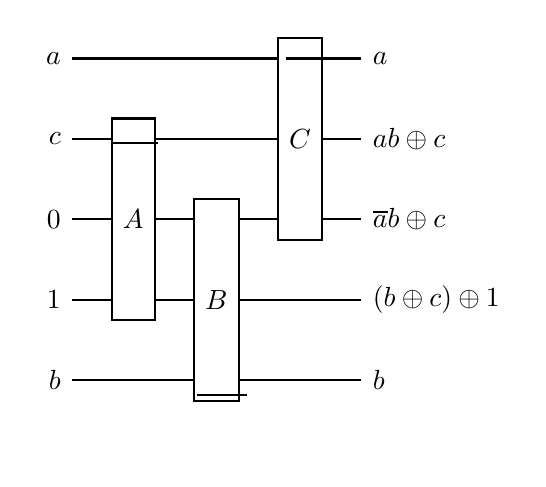
\begin{tikzpicture}
            \node[scale=1.0] {
                \begin{quantikz}[execute at
                    end picture={
                        \draw[thick]
                        ([yshift=0.0pt, xshift=77.0pt]\tikzcdmatrixname-1-1.north west)--
                        ([yshift=0.0pt, xshift=95.0pt]\tikzcdmatrixname-1-1.north west);
                        \draw[thick]
                        ([yshift=-30.43pt, xshift=14.0pt]\tikzcdmatrixname-1-1.north west)--
                        ([yshift=-30.43pt, xshift=31.0pt]\tikzcdmatrixname-1-1.north west);
                        \draw[thick]
                        ([yshift=-121.70pt, xshift=45.0pt]\tikzcdmatrixname-1-1.north west)--
                        ([yshift=-121.70pt, xshift=63.0pt]\tikzcdmatrixname-1-1.north west);
                    }]
                    \lstick{$a$} & \qw         & \qw          & \gate[3]{C} & \qw \rstick{$a$} \\
                    \lstick{$c$} & \gate[3]{A} & \qw          & \qw         & \qw \rstick{$ab \oplus c$} \\
                    \lstick{$0$} & \qw         & \gate[3]{B}  & \qw         & \qw \rstick{$\overline{a}b \oplus c$} \\
                    \lstick{$1$} & \qw         & \qw          & \qw         & \qw \rstick{$(b \oplus c) \oplus 1$} \\
                    \lstick{$b$} & \qw         & \qw          & \qw         & \qw \rstick{$b$} \\
                \end{quantikz}
            };
        \end{tikzpicture}
    \end{center}
    As we can see, the $A$, $B$ and $C$ Fredkin gates all in all create a Toffoli gate on the first wire as $a$, last wire as $b$ and second wire as $ab \oplus c$.

    To create a Fredkin gate from Toffoli gates, the least amount of gates needed is 3, and the least amount of ancilla bits needed is 0.
    \begin{center}
        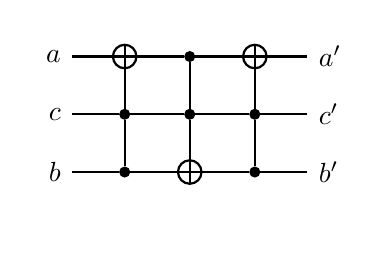
\begin{tikzpicture}
            \node[scale=1.0] {
                \begin{quantikz}
                    \lstick{$a$} & \targ{}   & \ctrl{1} & \targ{}   & \qw \rstick{$a'$} \\
                    \lstick{$c$} & \ctrl{-1} & \ctrl{1} & \ctrl{-1} & \qw \rstick{$c'$} \\
                    \lstick{$b$} & \ctrl{-1} & \targ{}  & \ctrl{-1} & \qw \rstick{$b'$} \\
                \end{quantikz}
            };
        \end{tikzpicture}
    \end{center}
    We can check, that this really is a Fredkin gate by calculating each case.

    \newpage

    \bibliographystyle{plain}
    \bibliography{references}

\end{document}
